% biomsample.tex
%
% v1.0 released 12th December 2006 (Dr. S. Sharma, Prof. N. Saxena, and Dr. S. Tahir)
%
% The biomsample.tex file has been amended to highlight
% the proper use of LaTeX2e code with the class file
% and using natbib cross-referencing.
%
\documentclass[useAMS,usenatbib, galley]{biom}
%\documentclass[useAMS,usenatbib,referee]{biom}
%
%
%  Papers submitted to Biometrics should ALWAYS be prepared
%  using the referee option!!!!
%
%
% If your system does not have the AMS fonts version 2.0 installed, then
% remove the useAMS option.
%
% useAMS allows you to obtain upright Greek characters.
% e.g. \umu, \upi etc.  See the section on "Upright Greek characters" in
% this guide for further information.
%
% If you are using AMS 2.0 fonts, bold math letters/symbols are available
% at a larger range of sizes for NFSS release 1 and 2 (using \boldmath or
% preferably \bmath).
%
% The usenatbib command allows the use of Patrick Daly's natbib package for
% cross-referencing.
%
% If you wish to typeset the paper in Times font (if you do not have the
% PostScript Type 1 Computer Modern fonts you will need to do this to get
% smoother fonts in a PDF file) then uncomment the next line
% \usepackage{Times}

\usepackage[figuresright]{rotating}

\usepackage{mathrsfs}
\usepackage{amsmath, bm}
\usepackage{natbib}
\usepackage{url}
\usepackage[outdir=./]{epstopdf}
\usepackage{array,longtable}
\usepackage{lscape}
\usepackage{float}  % PUT FIGURE HERE
\usepackage{array}  % fix column width 	
\usepackage{caption}
\captionsetup[figure]{labelfont=bf}
\captionsetup[table]{labelfont=bf}
\usepackage{multirow}
\usepackage{booktabs} % Create TABS
\usepackage{supertabular,booktabs}
%%%%% AUTHORS - PLACE YOUR OWN MACROS HERE %%%%%

%  If you have a landscape table you need to use the rotating package

%% \raggedbottom % To avoid glue in typesetteing, sbs>>
\newcommand{\OurMethod}{MEQLEA}
\newcommand{\HowmanyTest}{six}
\newcommand{\aaCase}{a}
\newcommand{\aCase}{b}
\newcommand{\cCase}{c}
\newcommand{\eCase}{d}
\newcommand{\fCase}{e}
\newcommand{\CMR}{CAMERA-rank}
\newcommand{\CMT}{CAMERA-modt}
\newcommand{\gent}{SigPathway}
\newcommand{\gen}{geneSetTest}
\newcommand{\genr}{MRSGE}
\newcommand{\thepapertobefinished}{Zhuo and Di, unpublished work}
\newcommand{\HowmanySimu}{$1,000$}


\newcolumntype{M}[1]{>{\centering\arraybackslash}m{#1}}
%%%%%%%%%%%%%%%%%%%%%%%%%%%%%%%%%%%%%%%%%%%%%%%%

\setcounter{footnote}{2}

\title[This is an Example of Recto Running Head]{Accounting for correlations in competitive gene set test for improved interpretation of genome-scale data}

\author{Bin Zhuo$^{*}$\email{zhuob@oregonstate.edu} \\
	   Department of Statistics, Oregon State University, Corvallis, OR, 97333
	   \and 
	   Duo Jiang$^{*}$\email{jiangd@stat.oregonstate.edu}\\
	    Department of Statistics, Oregon State University, Corvallis, OR, 97333
	   }

\begin{document}

%\date{{\it Received October} 2004. {\it Revised February} 2005.\newline 
%{\it Accepted March} 2005.}

%\pagerange{\pageref{firstpage}--\pageref{lastpage}} \pubyear{2006}

%\volume{59}
%\artmonth{December}
%\doi{10.1111/j.1541-0420.2005.00454.x}

%  This label and the label ``lastpage'' are used by the \pagerange
%  command above to give the page range for the article

\label{firstpage}

%  pub the summary here

\begin{abstract}
Competitive gene set test is a widely used tool for interpreting high-throughput biological data, such as gene expression and proteomics data. It aims at testing categories of genes for enriched association signals in a list of genes inferred from genome-wide data. Most conventional enrichment testing methods ignore or do not properly account for the widespread correlations among genes, which, as we show, can result in inflated type I error rates and power loss. We propose a new framework, \OurMethod, for gene set test based on a mixed effects quasi-likelihood model, where the data are not required to be Gaussian. Our method effectively adjusts for completely unknown, unstructured correlations among the genes. It uses a score test approach and allows for analytical assessment of $p$-values. Compared to existing methods such as GSEA and CAMERA, our method enjoys robust and substantially improved control over type 1 error and maintains good power in a variety of correlation structure and association settings. We also present two real data analysis to illustrate our approach.
\end{abstract}

%
%  Please place your key words in alphabetical order, separated
%  by semicolons, with the first letter of the first word capitalized,
%  and a period at the end of the list.
%

\begin{keywords}
%Colostrum; Milk; Milk oligosaccharide; Non-human mammal.
\end{keywords}

\maketitle

	\section{Introduction}\label{section:introduction}
	
	\textbf{What is enrichment analysis? Why would people care about that?}\\
	\textit{Gene set test} is a statistical framework of studying the association between a test set---a \textit{prior} set of biologically related genes---and a set of genes that are significantly correlated with treatment or experimental design variables. A key task of gene expression analysis involves the detection of differentially expressed genes. Differential expression (DE) analysis  evaluates each individual gene separately, and therefore it fails to provide insight into the relation between treatment variables and the prior gene set under study. Gene set test helps researchers better understand the underlying biological processes in terms of ensembles of genes.
	
	\textbf{What are the differences between self-contained and competitive test? And how does they work?}\\
	Depending on the definition of the null hypothesis, there are two types of gene set test: the \textit{self-contained} test and the \textit{competitive} test \citep{goeman2007analyzing}. A self-contained test examines a set of genes by a fixed standard without reference to other genes in the genome (see, for example, \cite{goeman2004global,goeman2005testing, tsai2009multivariate, wu2010roast, huang2013gene}). A competitive test compares DE
	genes in the test set to those not in the test set \citep{tian2005discovering, wu2012camera, yaari2013quantitative}. Many methods, regardless of the type of test, perform a three-stage analysis \citep{khatri2012ten}: on the first stage, a \textit{gene-level statistic} is calculated for each gene in the whole genome to measure the association between the expression profiles and the experimental design variables; such gene-level statistic includes, among others, \textit{signal-to-noise ratio} \citep{subramanian2005gene},\textit{ordinary $t$-statistic} \citep{tian2005discovering} or \textit{moderated $t$-statistic} \citep{Smyth2004moderated}, \textit{log fold change} \citep{kim2005page} and \textit{$Z$-score} \citep{efron2007correlation}. On the second stage, a \textit{set-level statistic} is obtained by utilizing the gene-level statistics from the first stage and their membership with respect to the test set (i.e., whether the gene belongs to the test set). Examples of the set-level statistic are \textit{enrichment score} \citep{subramanian2005gene}, \textit{maxmean statistic} \citep{efron2007testing}, and statistic derived from joint distribution of gene-level statistics \citep{yaari2013quantitative}, to name a few. On the third stage, a $p$-value is assigned to the test set by comparing the set-level statistic to its reference distribution. The competitive gene set test is much more popular among genomic literatures \citep{goeman2007analyzing, gatti2010heading}.  
	
	%Competitive gene set test \citep{goeman2007analyzing} is a gene expression analysis that compares differential expression (DE) for genes in the test set to that for genes not in the test set. Most competitive gene set tests, as described by \cite{barry2008statistical}, are typically two-stage procedures:  on the second stage, a $p$-value is reported from the The test set may represent biological pathways or network, or some other grouping based on biological knowledge. Incorporating such prior information of the grouping makes it easier for biologists to interpret the results of DE analysis.
	
	\textbf{Independent gene set test} \\
	Many competitive gene set tests rely on independence of gene-level statistics which further depends on independence among genes. Those tests are parametric or rank-based procedures that assume the gene-level statistics to be independent and identically distributed, or gene permutation procedures that generate the same approximate null for the set-level statistics. For example, PAGE  \citep{kim2005page} conducts one-sample $z$-test by comparing the mean of gene-level statistics (i.e., the mean of log fold changes) in the test set to a normal distribution under the null. The $2\times 2$ contingency-table-based tests examine the significance of the test set by dichotomizing the outcomes of DE analysis and cross-classifying the genes according to whether they are indicated as DE and whether they are in the test set (see \cite{huang2009bioinformatics} for a review and references therein). sigPathway \citep{tian2005discovering} and ``\gen" in the limma package \citep{Smyth2004moderated} evaluate the set-level $p$-values by permuting gene labels. However, tests assuming independence of genes may result in inflated false discovery rate \citep{efron2007testing,goeman2007analyzing, gatti2010heading,wu2012camera,yaari2013quantitative}, as genes within a gene set are often co-expressed and function together.
	
	\textbf{Tests that account for inter-gene correlation}\\
	A handful of methods have been proposed to account for inter-gene correlation in competitive gene set test. One attempt is to evaluate the set-level statistic by permuting the biological sample labels (see, for example, \cite{subramanian2005gene, efron2007testing}). Permuting sample labels does not require an explicit understanding of the underlying correlation structure among genes and thus protects the test against such correlation. Since permuting sample labels is computationally inefficient, \cite{zhou2013empirical} proposed an analytic approximation to permutations for set-level score statistics, which preserves the essence of permutation gene set analysis with greatly reduced computational burden. However, an unavoidable problem arising from sample permutation approach is that it implicitly alters the null hypothesis being tested and it is therefore difficult to characterize the null and the alternative hypotheses \citep{goeman2007analyzing, khatri2012ten, wu2012camera}. Another attempt is to use set-level statistic that directly includes inter-gene correlation estimated from the data. For example, CAMERA \citep{wu2012camera} calculates a \textit{variance inflation factor} (VIF) from sample correlation (after the treatment effect removed), and then incorporates it into their set-level statistics to account for inter-gene correlations. A recent extension to CAMERA,  QuSAGE \citep{yaari2013quantitative}, also used the same VIF to adjust for inter-gene correlations but includes the VIF in a different set-level statistic. The VIF is a crucial factor and valid estimation of it relies on the assumption that correlation between any two local statistics are almost the same as correlation between their corresponding expression profiles. This assumption has been demonstrated (??? a better word???) by simulation \citep{barry2008statistical} for several gene-level statistics (e.g., $t$-statistic, Wald-type statistic for regressing expression on censored time-to-event data through a Cox proportional hazards model). However, this assumption holds only for the case where all the hypotheses are under the null (i.e., no gene is DE), and the correlation among gene-level statistics (e.g., $t$-statistics) can be badly estimated by sample correlation when a fraction of genes are DE (\thepapertobefinished). 
	% The CAMERA procedure thus may be too conservative for controling type I error in the presence of DE genes, as will be demonstrated in our simulation study. 
	
	
	% (This is a self-contained gene set test) \cite{huang2013gene} uses a multivariate linear regression model in which the inter-gene correlation are explicitly modeled by a working covariance matrix. 
	
	\textbf{What do we propose?} \\
	We propose a new framework for enrichment analysis that we will call Mixed Effects Quasi-Likelihood Enrichment Analysis (\OurMethod). Our strategy is to avoid the discrepancy between correlations among expression profiles and those among gene-level statistics caused by the presence of DE genes. Instead, we use differences in mean as gene-level statistics for a two group comparison experiment. We model the covariance of gene-level statistics by two variance components, one attributable to correlations among samples after treatment effect removed, and the other attributable to the DE effect associate with the treatment. The benefit of quasi-likelihood is that the data are not required to be Gaussian. Our method effectively adjusts for completely unknown, unstructured correlations among the genes. \OurMethod~uses a score test approach and allows for analytical assessment of $p$-values. Compared to existing methods including GSEA and CAMERA, \OurMethod~enjoys robust and improved control over type I error and maintains good power in a variety of correlation structure and association settings. 
	
	\textbf{What is the plan of this paper?} \\
	The rest of the paper is organized as follows: in Section \ref{section:methods} we describe the methodology and then the simulation setup of \OurMethod, and summarize related existing methods; in Section \ref{section:results} we present results from comparison of \OurMethod~to other existing methods by simulation study, and illustrate the application of our method by two real data sets; in Section \ref{section:conclusion} we conclude and also specifies the future work.

	
	
	\section{Methods}\label{section:methods}
	We consider a gene expression (e.g. RNA-Seq or microarray) experiment, in which we compare the gene expression profiles of samples from two groups: a treatment group with $n_1$ samples referred to as ``cases" and a control group with $n_2$ samples referred to as ``controls" ($n_1,n_2\ge 3$). Suppose the expression profiles of a set of $m$ genes are observed for each sample. An unknown subset of these genes are DE between cases and controls, with varying sign and magnitude of DE effects. The genes are also allowed to have (negatively or positively) correlated expression profiles. In enrichment analysis, we are interested in a pre-defined set of genes, for example, from a known pathway or given by a functional annotation term from a database such as KEGG \citep{kanehisa2000kegg} or GO \citep{ashburner2000gene}. Our goal is to test whether this known gene set is enriched with differential expression signals. Let $\bm G$ be an $m$-dimensional vector defining the gene set of interest, where $G_i=1$ if and only if the $i^{th}$ gene is in the set and $G_i=0$ otherwise. Our analysis will condition on $\bm G$ and test if $\bm G$ is associated with enhanced DE effects. In the following sections, we will first construct a hierarchical model for the gene expression data incorporating possible correlations among the $m$ genes, from which we will derive a quasi-likelihood model for the gene-level DE statistics jointly for all the genes. Based on this model, we will then present our enrichment test, and discuss its connections with CAMERA. Finally, we will describe our simulation studies used to evaluate our method. For the rest of \textbf{Methods}, our presentation of the method is conditional on $\bm G$ unless otherwise indicated.
	
	\subsection{\OurMethod}
	\subsubsection{A hierarchical model for the gene expression data}\label{subsection:YModel}
	We will start by presenting the hierarchical model for the observed gene expression data, which will incorporate the following features. 
	Firstly, for a given sample, the expression profiles of different genes are allowed to be correlated. We further assume that the correlation structure is the same across samples. Secondly, different genes may have different baseline expression profiles, where ``baseline" refers to the average among controls. Thirdly, for any given gene, its mean expression profile in the treatment group can be either higher, lower or the same compared to the control group, depending on whether the gene is up-regulated, down-regulated, or not DE. For the genes that are differentially expressed, their DE effects are modeled additively and are allowed to have heterogeneous signs and magnitudes. Finally, given a gene, and its DE effect, the expression profile is allowed to vary independently across samples, which captures measurement error and sample-level variability.
	
	To present our model formally, we first introduce some notation. Let $n=n_1+n_2$ be the total sample size. Let $\bm X$ be an $n$-dimensional known vector of 1's and 0's denoting the case-control membership of the samples, with $X_i=1$ for a case and $X_i=0$ for a control. Let $\bm Y$ be an $n$ by $m$ matrix representing the expression data, in which each row is the expression profile for a sample and $Y_{ij}$ ($1\le i\le n, 1\le j\le m$) is the expression profile of sample $i$ at gene $j$. Let $\mu_j$ ($1\le j\le m$) be the baseline expression profile for gene $j$. $\mu_j$'s are treated as nuisance parameters and as we will see later do not contribute to our analysis. Let $\bm \Delta=(\Delta_1, \cdots, \Delta_m)^T$ be a vector for the additive DE effects for the genes. Gene $j$ is not DE if $\Delta_j=0$, up-regulated if $\Delta_j >0 $ and down-regulated if $\Delta_j<0$. We model $\bm \Delta$ as a random effect, for which we will detail our assumptions later. Given $\mu_j$ and $\Delta_j$, the mean expression profile for the control group and the treatment group are $\mu_j$ and $\mu_j+\Delta_j$, respectively. Given these means, the noise in the observed expression data for the $i^{th}$ sample is denoted by the mean zero error vector $\epsilon_i=(\epsilon_{i1},\cdots,\epsilon_{im})^T$, $1\le i\le n$. We assume $\bm\epsilon:=(\epsilon_1,\cdots,\epsilon_m)$ to be independent of $\bm \Delta$ and to have mean zero. Without loss of generality, we also assume $\mbox{Var}(\epsilon_{ij})=1$ for all genes and samples. For a real gene expression data set typically not satisfying this assumption, we can standardize the data by each gene to ensure its empirical variance equals one before implementing our method. For the covariance structure of $\epsilon$, we assume 
	\begin{gather}
		\text{$\epsilon_{i_1}$ and $\epsilon_{i_2}$ are independent, \;\;$i_1\ne i_2$},\label{eq:gene_indep}\\
		\mbox{Cov}(\epsilon_i|\bm G)=\bm C, \;\;1\le i\le n,\label{eq:gene_cor}
	\end{gather}
	where $\bm C$ is an $m$ by $m$ inter-gene correlation matrix shared by all samples. $\bm C$ is generally unknown.
	
	Putting these elements together, we obtain the following model for the expression data $\bm Y$ given $\bm X$ and $\bm G$ 
	\begin{align}
		\label{eq:Ymodel}
		Y_{ij} = \mu_j + X_i\cdot\Delta_j + \epsilon_{ij},
	\end{align}
	for $1\le i\le n, 1\le j\le m$. $\bm G$ enters this model via $\Delta_j$ and possibly $\mu_j$.
	
	\subsubsection{Assumptions on the DE effects $\Delta_j$}\label{subsection:DeltaModel}
	Conditional on $\bm G$, we assume that the $\Delta_j$'s are mutually independent and come from either of the two distributions, $\mathscr{D}_1$ and $\mathscr{D}_2$, depending on whether $G_j=0$ or 1. We denote the expected values of $\mathscr{D}_1$ and $\mathscr{D}_2$ by $\beta_0$ and $\beta_0+\beta_1$, respectively, and their variances by $\sigma_1^2$ and $\sigma_2^2$, respectively. It follows that 
	\begin{equation}
		\label{eq:Delta}
		E(\bm \Delta|\bm G)=\beta_0 + \beta_1 \bm G,\;\; \mbox{var}(\bm \Delta|\bm G) = \sigma_1^2\bm I_1+\sigma_2^2\bm I_2,
	\end{equation} 
	where $\bm I_1$ and $\bm I_2$ are diagonal matrices of dimension $m$ with $0$'s and $1$'s on their diagonals. The $1$'s in the diagonal of $\bm I_1$ correspond to the genes with $G_j=1$ and those for $\bm I_2$ to the genes with $G_j=0$.
	
	Aside from the conditions in Equation (\ref{eq:Delta}) on the first two moments, we do not impose any specific distributional assumptions such as normality on $\bm \Delta$. For example, the distribution of a given $\Delta_j$ can put positive mass on zero, which allows for the highly likely event that some of the genes are not DE. To further motivate our general framework for $\bm \Delta$, we present a simple model included by Equation (\ref{eq:Delta}) as a special case. Suppose the $m$ genes are independently sampled to be either DE or not. The probability for gene $j$ to be DE is $p_t$ if $G_j=1$ or $p_b$ if $G_j=0$. For DE genes, their DE effects are sampled independently from a common distribution with mean $\mu_\delta$ and variance $\sigma^2_\delta$. Under these assumptions, 
	\begin{equation}
		\label{eq:DeltaBinom}
		E(\Delta_j|\bm G) = p_j\mu_{\delta},\;\; \mbox{var}(\Delta_j|\bm G)= p_j\sigma_{\delta}^2 + p_j(1-p_j)\mu_{\delta}^2,
	\end{equation}
	where $p_j=p_{t}$ if $G_j=1$ and $p_j=p_{b}$ if $G_j=0$. It can be shown that this model is a special case of Equation (\ref{eq:Delta}).
	
	\subsubsection{Model for gene-level statistics}\label{subsection:UModel}
	For each gene $j$, we consider the DE statistic (gene-level statistic???) given by 
	\begin{equation}
		\label{eq:U}
		U_j = \dfrac{\sum_{i: X_i=1}Y_{ij}}{n_1} - \dfrac{\sum_{i: X_i=0}Y_{ij}}{n_2},
	\end{equation}
	which is sample mean difference in the expression profile between cases and controls. Given our assumption that $\epsilon_j$ has variance 1, $U_j$ provides a DE metric for gene $j$. We will construct a quasi-likelihood model for $\bm U=(U_1,\cdots,U_m)^T$ by deriving the mean and covariance structures of $\bm U$ from the model for $\bm Y$ described in Sections \ref{subsection:YModel} and \ref{subsection:DeltaModel}. We first observe that combining Equations (\ref{eq:U}) and (\ref{eq:Ymodel}) yields
	\begin{equation} 
		U_j = \Delta_j + \eta_j, \text{where } \eta_j = \dfrac{1}{n_1}\sum_{i: X_i=1}\epsilon_{ij}- \dfrac{1}{n_1}\sum_{i: X_i=0}\epsilon_{ij}.
	\end{equation}
	It can be shown based on Equations (\ref{eq:gene_indep}), (\ref{eq:gene_cor}) and (\ref{eq:Delta}) that
	\begin{gather}
		E(\bm U|\bm G) = \beta_0+\beta_1 \bm G,\label{eq:U_mean}\\
		\Sigma:=\mbox{var}(\bm U|\bm G) = \sigma_0^2\bm C + \sigma_1^2\bm I_1+\sigma_2^2\bm I_2,\label{eq:U_var}
	\end{gather}
	where $\sigma_0^2=1/n_1+1/n_2$ is a known parameter. We note that in Equation (\ref{eq:U_var}), the covariance structure of $\bm U$ has three components, a component with $\bm C$ which accounts for the contribution from sample-level noise $\bm \epsilon$, and two additional components from the DE effect $\bm \Delta$. It is noteworthy that both the $\bm C$ component and the $\bm \Delta$ components contribute to the variance of $U_j$'s, whereas only the $\bm C$ component contributes to the correlation among $U_j$'s.
	
	\subsubsection{The set-level test statistic}\label{subsection:MEQL}
	For a competitive gene set test, it is often unclear what the hypothesized null is and what is being tested \citep{barry2008statistical,wu2012camera}. In our approach, to detect patterns of the DE signals in the gene set of interest that stand out compared with genes not in the set, we test $H_0: \mathscr{D}_0=\mathscr{D}_1$ against $H_1: \mathscr{D}_0\ne\mathscr{D}_1$. For example, for the special scenario given by Equation (\ref{eq:DeltaBinom}), this amounts to testing $p_{b}=p_{t}$ against $p_{b}\ne p_{t}$.
	To construct the test statistic, we focus on the part of the alternative space where $E(\mathscr{D}_0)\ne E(\mathscr{D}_1$), or equivalently $\beta_1\ne 0$. We first consider the less interesting case with uncorrelated genes, in which $\bm C$ equals $\bm I$, an $m$-dimensional identity matrix. Under the quasi-likelihood model for $\bm U$ given in Section \ref{subsection:UModel},  the quasi-score statistic for $\beta_1$ has the form $S \propto \bm G^T(\bm U-\hat\beta_0\bm 1_m)$, where $\hat\beta_0=\overline{U}$ is an estimate for $\beta_0$ and $\bm 1_m$ is a $m$-dimensional vector of 1's. To perform a quasi-score test, one would divide $S^2$ by its estimated variance under $H_0$ and the assumption that $\bm C=\bm I$. The resulting test statistic is 
	\begin{equation}
		T_{\text{u}} = \dfrac{S^2}{\widehat{\mbox{Var}}_{0, \bm C=\bm I}(S|\bm G)} = \dfrac{[\bm G^T(\bm U-\hat\beta_0)\bm 1_m]^2}{\bm G^T(\bm I-\bm H)\bm G}, 
	\end{equation}
	where $\bm H = \dfrac{1}{n}\bm 1_m\bm 1_m^T$. The subscript ``u" stands for ``uncorrelated genes." For the case of interest when inter-gene correlation is present, $\bm C$ is a non-trivial correlation (???Covariance) matrix. We will again form our test statistic based on $S$. But for the denominator of the statistic, the null variance of $S$ will be evaluated under the quasi-likelihood model with non-trivial $\bm C$. By Equation (\ref{eq:U_var}), the variance of $S$ is given by $\mbox{Var}(S|\bm G) = \bm G^T(\bm I-\bm H)\Sigma(\bm I-\bm H)\bm G$. Note that $H_0: \mathscr{D}_0=\mathscr{D}_1$ implies $\sigma_1^2=\sigma_2^2$. Thus, under $H_0$, $\Sigma:=\mbox{Var}_{0}(\bm U|\bm G)=\sigma_0^2\bm C+\sigma_1^2\bm I$, where $\sigma_0=1/n_1+1/n_2$ is known and $\sigma_1^2$ is an unknown parameter. To estimate $\sigma_1^2$ under $H_0$, we observe that $\mbox{var}_{0}(U_j)=\sigma_0^2+\sigma_1^2$ and use $\hat\sigma_1^2=\sum_{j=1}^m(U_j-\overline{U})^2/(m-1)-\sigma_0^2$. Therefore, assuming $\bm C$ is known, we can obtain the \OurMethod~test statistic given by
	\begin{equation}
		T = \dfrac{S^2}{\widehat{\mbox{Var}}_{0}(S|\bm G)} = \dfrac{[\bm G^T(\bm U-\hat\beta_0\bm 1_m)]^2}{\bm G^T(\bm I-\bm H)\hat{\bm\Sigma}(\bm I-\bm H)\bm G}, 
	\end{equation}
	where $\hat{\bm\Sigma}=(1/n_1+1/n_2)\bm C+\hat\sigma_1^2\bm I$ is a null estimate of $\bm \Sigma$. Under suitable regularity conditions, significance of the test could then be assessed by comparing $T$ to a $\chi^2_1$ distribution.
	
	In practice, the inter-gene covariance matrix $\bm C$ is usually unknown. So we substitute $\bm C$ with $\hat {\bm C}$, the empirical covariance matrix of the expression data after controlling for possible DE effects by centering the expression profiles of cases and controls separately around zero. Formally, $\hat {\bm C}$ is given by $\hat C_{jk}=\dfrac{1}{n}\sum_{i=1}^n(Y_{ij}-\alpha_{ij})(Y_{ik}-\alpha_{ik})$ where $\alpha_{ij}=\sum_{i':X_{i'}=X_{i}}Y_{i'j}/\sum_{i'=1}^n1\{X_{i'}=X_{i}\}$ is the average expression profile at gene $j$ for all samples from the same group (either treatment or control) as sample $i$. In real data sets, the number of genes, $m$, is usually much greater than the sample size $n$, in which case $\bm C$ is a high-dimensional parameter that cannot be efficiently estimated by $\hat {\bm C}$. Interestingly, however, we find (note???) that the the test statistic $T$ relies not on the accurate estimation of the entire $\bm C$, but only on three parameters involving $\bm C$, which can be much more realistically estimated by a moderate sample size. To demonstrate this, we re-arrange the order of the rows and columns of $\bm C$ to allow the partition $\bm C=\left[\begin{array}{cc}
	\bm C_{11} & \bm C_{12} \\       \bm C_{12}^T & \bm C_{22} \\      \end{array}\right] $,
	where $\bm C_{11}$ is the correlation matrix for genes in the test set, $\bm C_{22}$ is that for gene in the background set (i.e., the complement of the test set), and $\bm C_{12}$ is the cross-correlation matrix between the two classes of genes. (To be continued....)

	
	
%	\subsection{Connection to current methods}
%	\OurMethod~...
%	CAMERA incorporates a VIF in their set-level statistics to account for inflation due to the presence of inter-gene correlation. \OurMethod is closely related to their approach in that set-level statistic in (REF)    
	
%	\subsection{Other competitive gene set tests}
	\subsection{Simulation Methods}
	
		\subsubsection{Simulation Setup}\label{subsection:simulation}
		In this section, we present results from type I error and power simulations. Since a standardization procedure is required by \OurMethod~for preprocessing data, we will simulate the standardized expression profiles for method illustration purpose. 
		
		Let $Y_{i}$ be the expression profile of gene $i$ and $\text{Cov}(Y_{i_1}, Y_{i_2})=\rho_{i_1, i_2}$ for any two genes $i_1$ and $i_2$. We assume that $\text{Cov}(Y_{i_1}, Y_{i_2})= \rho_1$ if genes $i_1$ and $i_2$ are both from the test set (i.e., $G_{i_1} = G_{i_2}=1$),  $\text{Cov}(Y_{i_1}, Y_{i_2}) =\rho_2$ if they are both from the background set (i.e., $G_{i_1} = G_{i_2}=0$), and  $\text{Cov}(Y_{i_1}, Y_{i_2})= \rho_3$ if $i_1$ is from the test set and $i_2$ is from the background set (i.e., $G_{i_1} =1,  G_{i_2}=0$). We examine five different correlation structures, listed as follows:
		
		\begin{enumerate}
			\item[(\aaCase):] $\rho_1 = \rho_2 = \rho_3 = 0$; that is, the genes are independent of each other.
			\item[(\aCase):] $\rho_1 = 0.1$, $\rho_2 = \rho_3 = 0$; that is, only the genes in the test set are correlated.
			\item[(\cCase):] $\rho_1 = \rho_2 = \rho_3 = 0.1$; that is, all genes are correlated, with an exchangeable correlation structure. 
			\item[(\eCase):] $\rho_1 = 0.1$, $\rho_2 = 0.05$, $\rho_3 = 0$; that is, 
			genes are correlated within the test set and within the background set, but any two genes, one from the test set and the other from the background set, are independent.
			\item[(\fCase):] $\rho_1 = 0.1$, $\rho_2 = 0.05$, $\rho_3 = -0.05$; that is, all genes are correlated, but the correlation between two genes depend on whether they belong to the test set or not.
			%	\item[(g):] genes are correlated in the same way as those from a real data.
		\end{enumerate}
		
		The simulations run as follows: first, we generate an entire gene set containing $m=500$ genes, from which we randomly sample $m_1 = 100$ genes to represent those in the test set, and the remaining $m_2=400$ genes those in the background set; second, for gene $i=1, \ldots, m$, we set the DE size $\delta_i$ to be $1$ and simulate the DE indicator $Z_i$ from $\text{Binom}(1, p_i)$,  where $p_i= p_t$ if gene $i$ belongs to the test set and $p_i = p_b$  otherwise, and then the DE effect $\Delta_i$ is the product of $Z_i$ and $\delta_i$; third, we set the ``true" mean expression values $\bm \mu_1 = \bm 0_m$ and $\bm \mu_2 = \bm \Delta$, respectively,  for the control and treatment groups; fourth, we simulate $n_1$ samples from $\text{MVN}(\bm \mu_1, \bm \Sigma)$ for the control group and $n_2$ samples from $\text{MVN}(\bm \mu_2, \bm \Sigma)$ for the treatment group, where the covariance $\bm \Sigma = \left[\text{Cov}(Y_{i_1}, Y_{i_2})\right]_{m\times m}$ may be one of the correlation structures in (\aaCase)-(\fCase).
		
		We have mentioned in the Introduction part that the test statistics correlations among genes are not equal to their sample correlations when at least one gene is truly DE (under two sample $t$-test???). Therefore, if there are true DE genes in the entire gene set, approaches assuming almost equality of correlations among gene-level statistics and those among expression values may not perform well. To illustrate this point, we performed two groups of simulations for each of  (\aaCase)-(\fCase) correlation structures. In both type I error and power simulations, we set the DE probability to be $0\%$ in group $A_1$ and $10\%$ in group $A_2$ for genes in the background set. In the type I error simulation, we have $p_t = p_b$ under the null. In the power simulation, we considered four different alternative scenarios $S_1$-$S_4$: for genes in the test set, we set DE probability to be $5\%, 10\%, 15\%$ and $20\%$ in group $A_1$, and $15\%, 20\%, 25\%$ and $30\%$ in group $A_2$. Table \ref{table:simusetup} summarizes the simulation setup for the two groups.
		
		% In both groups of simulation, we fixed the DE size $\delta$ for each alternative and the six different correlation structures. 
		
		% (summarized in Table \ref{table:simusetup} ): we simulated expression data with no DE genes in group $A_1$, that is, $p_b = 0$; and in group $A_2$, we simulated data sets with the same DE probabilities for all genes---specifically, DE probabilities are the same for genes in the test set and for those in the background set with $p_t= p_b = 0.2$. 
		
		
		\begin{table}[!ht]
			\centering
			\caption{Parameter setup for type I error and power simulations. $S_0$ repersents scenario for type I error simulation. $S_1$-$S_4$ represent the four alternatives regarding power simulation.}
			\begin{tabular}{rp{1cm}p{1cm}p{1cm}p{1cm}p{1cm}}
				\hline\hline
				% 		& \multicolumn{6}{c}{Simulation} \\
				%		\cline{2-7}
				Group & $p_b$ &  \multicolumn{4}{c}{$p_t$}  \\ 
				\cline{3-6}
				& $S_0$  & $S_1$ & $S_2$ & $S_3$ & $S_4$\\ 
				\hline
				$A_1$ & 0\%   & 5\% & 10\% & 15\% & 20\%\\ 
				$A_2$ & 10\%  & 15\%& 20\%& 25\% & 30\%\\ 
				\hline\hline
				\multicolumn{6}{p{8cm}}{$p_b$: DE probablility for genes in the background set. }	 \\	
				\multicolumn{6}{p{8cm}}{$p_t$: DE probablility for genes in the test set. }	 \\	
			\end{tabular}
			\label{table:simusetup}
		\end{table}
	
		\subsubsection{Other methods considered}
		
		We will compare \OurMethod~to~\HowmanyTest~existing gene set tests: GSEA \citep{subramanian2005gene}, two versions of the CAMERA procedure ---\CMT~and \CMR~\citep{wu2012camera}, \gent~\citep{tian2005discovering}, MRSGE \citep{michaud2008integrative}, and QuSAGE \citep{yaari2013quantitative}. Except \gent~and MRSGE, all methods account for correlation among genes. GSEA calculates an enrichment score for the test set by examining the ranking (according to some metric, for example, signal-to-noise ratio) of its member genes, and determines the significance of the enrichment score by randomly permuting sample labels. \CMT~uses moderated $t$-statistics \citep{Smyth2004moderated} as gene-level statistics and estimate a VIF to account for inter-gene correlations in the set-level statistic, and \CMR~is the rank version of the \CMT. The \gent~is slightly different from its original version of \cite{tian2005discovering} in that it uses moderated $t$-statistics rather than the ordinary $t$-statistics as gene-level statistics. MRSGE is also known as the rank version of \gent~\citep{wu2012camera}. QuSAGE generates from $t$-test a probability density function (PDF) for each gene, combines the individual PDFs using convolution, and quantifies enrichment of the test set with a complete PDF. 
		
		
		For software implementation, GSEA is modified from the original R-GSEA script (\url{http://software.broadinstitute.org/gsea/index.jsp}) to accommodate single gene set test. CAMERA and \genr~are implemented in the limma package \citep{smyth2005limma} in the Bioconductor project \citep{gentleman2004bioconductor}, QuSAGE is available in the Bioconductor package of the same name, and \gent~is implemented by ourselves. Because GSEA and \OurMethod~do not support linear models, the implementations are restricted to two-group comparisons.
		
		
		%The \HowmanyTest~tests differ in one or more aspects, although all tests except QuSAGE follow the three-stage paradigm described in Section~\ref{section:introduction}. For GSEA, the gene-level statistics are the rankings of genes according to a ranking metric (we use signal-to-noise ratio, the default metric in R-GSEA throughout this paper), then based on the rankings an enrichment score for the test set is calculated, and the significance of the enrichment score is determined by randomly permuting the sample labels. Both \CMT~and \gent~use the moderated $t$-statistics \citep{Smyth2004moderated} as gene-level statistics, and determine whether the means of the gene-level statistics are significantly different for genes in the test set versus genes in the background set. The difference is how they evaluate the set-level statistics: \CMT~uses a $t$-statistic that allows the gene-level statistics in the test set to be correlated by first estimating a VIF, and then incorporating it into the $t$-statistic to adjust for inter-gene correlation (see materials and methods section of \cite{wu2012camera}); \gent~accesses the significance of the test set by comparing the observed set-level statistics to its null distribution generated by permuting gene labels. \CMR~and MRGSE conduct a Wilcoxon-Mann-Whitney rank sum test, and they amount to, respectively,  \CMT~and \gent~in that they compare the rankings instead of the gene-level statistics themselves for genes in the test set to those for genes in the background set. QuSAGE generates from $t$-test a probability density function (PDF) for each gene, combines the individual PDFs using convolution, and quantifies gene-set activity with a complete PDF. The complete PDF can be used to compare a baseline value for self-contained gene set test, or to compare differences in expression profiles between test set and background set in competitive gene set test.  
		
		In terms of type I error control and power, we expect some of the six tests to have different performances between group $A_1$ and $A_2$ simulations under one or more correlation structures. 
		 
	
	\section{Results}\label{section:results}
	
	According to the simulation setup in Section \ref{subsection:simulation}, the test set is not enriched if DE probabilities are the same for genes in the test set and for those in the background set (i.e., $p_t =0\%$ for group $A_1$ and $p_t = 10\%$ for group $A_2$), in which case we evaluate the type I error. As to power, we set DE probability according to each of alternative scenarios $S_1$-$S_4$ (see Table \ref{table:simusetup}) and calculate the proportion of data sets for which a test would reject at a given level $\alpha$. The results are based on \HowmanySimu~simulated data sets. 
		
		

	\subsection{Type I error simulations}\label{subsection:typeIerror}

	We report the type I error simulation results for group $A_1$ and $A_2$ simulations. Figure \ref{fig:typeIerror} shows the uniform quantile-quantile (QQ) plots of $p$-values for the seven~approaches (\OurMethod, \gent, \genr, \CMT, \CMR, GSEA and QuSAGE) under each of the five correlation structures. The left column of Figure \ref{fig:typeIerror} shows the $p$-values of group $A_1$ simulations. Each plot, from top to bottom, corresponds accordingly to correlation structures (\aaCase)-(\fCase). GSEA and \OurMethod~hold the size of type I error rate correctly for all five correlation structures, with simulated $p$-values uniformly distributed on $[0, 1]$. The two versions of CAMERA control type I errors correctly for correlation structures (\aaCase) and (\aCase), yet they are too conservative for the case of (\cCase) and anti-conservative for correlation structures (\eCase) and (\fCase). \gent~and \genr~procedures have well-calibrated type I error for correlation structures (\aaCase) and (\cCase), but are anti-conservative the case of (\aCase), (\eCase) and (\fCase). QuSAGE has good type I error control for only (\aCase), and is too conservative for (\aaCase), (\eCase) and (\fCase), and anti-conservative for (\cCase).
	
	The right column of Figure \ref{fig:typeIerror} shows type I error rate of group $A_2$ simulations. \OurMethod~continues to hold the size of type I error rate, whereas GSEA is skewed towards small $p$-values, under all five correlation structures. The two versions of CAMERA control type I error rate correctly for (\aaCase) where genes are simulated to be independent, but may liberal in other situations (conservative in (\aCase) (\cCase), and (\eCase), and slightly anti-conservative in (\fCase)). \gent, \genr~and QuSAGE have similar performances as they do, respectively, in group $A_1$ simulations.
	
	\textbf{Explain why this happens}\\
	\OurMethod~shows consistent accuracy for type I error control across all simulations, but the accuracy of the other \HowmanyTest~methods may be affected by two factors: the inter-gene correlation structures, and DE probability of each gene. \OurMethod~controls the size of type I error well because it uses difference in mean as gene-level statistic, and the correlations among gene-level statistics are fully reflected in sample correlation. GSEA evaluates the enrichment score of a test set by generating its null distribution from sample permutation. When there's no DE genes such as in the case of group $A_1$ simulations, GSEA performs extremely well since permuting sample labels won't change the underlying correlation structure. When DE genes exist, however, sample permutation will destroy the inter-gene correlation structure, which explains the complete failure of GSEA in controlling type I error for the case of group $A_2$ simulations. For CAMERA and QuSAGE, the VIF of the gene-level statistics (moderated $t$-test in \cite{wu2012camera}) may be over-estimated when a fraction of genes are DE (\thepapertobefinished), and therefore the set-level test statistic is under-estimated. The performances of those methods---QuSAGE and two versions of CAMERA---are subject to the underlying correlation structures. Moreover, the performance of CAMERA is complicated by the fact that the set-level statistic takes into account only the inter-gene correlation in the test set without addressing that in the background set.
	
	Different from the five methods mentioned above, \gent~and \genr~rely on independence between genes. It's not surprising that gene permutation method, such as \gent~and \genr, controls type I error correctly when genes are ``equally-correlated": in (\aaCase) genes are simulated to be independent, and in (\cCase) genes are simulated to have an exchangeable correlation structure. However, both \gent~and \genr~fail to hold type I error size for the remaining three correlation structures. These simulations show that even small inter-gene correlations will inflate the false discovery rate when the test does not account for inter-gene correlations.  
	
	%We note that both methods perform better in group $A_2$ as compared to their counterpart in group $A_1$ simulation under each of (\aCase), (\eCase) and (\fCase) correlation structures. In group $A_2$ where there are DE genes both in the test set and in the background set, the correlation between the gene-level statistics is smaller (in absolute value) than between sample correlation. Since the genes are simulated to be slightly correlated ($\rho_1=0.1, \rho_2 = 0.05, \rho_3 = -0.05$), the correlation between the gene-level statistics are almost negligible for \gen~procedure to work. 
	

\begin{figure*}[!th]
	\begin{center}
	
\includegraphics[width=20cm,height=0.6cm]{Figures/parallel_legend.eps}
	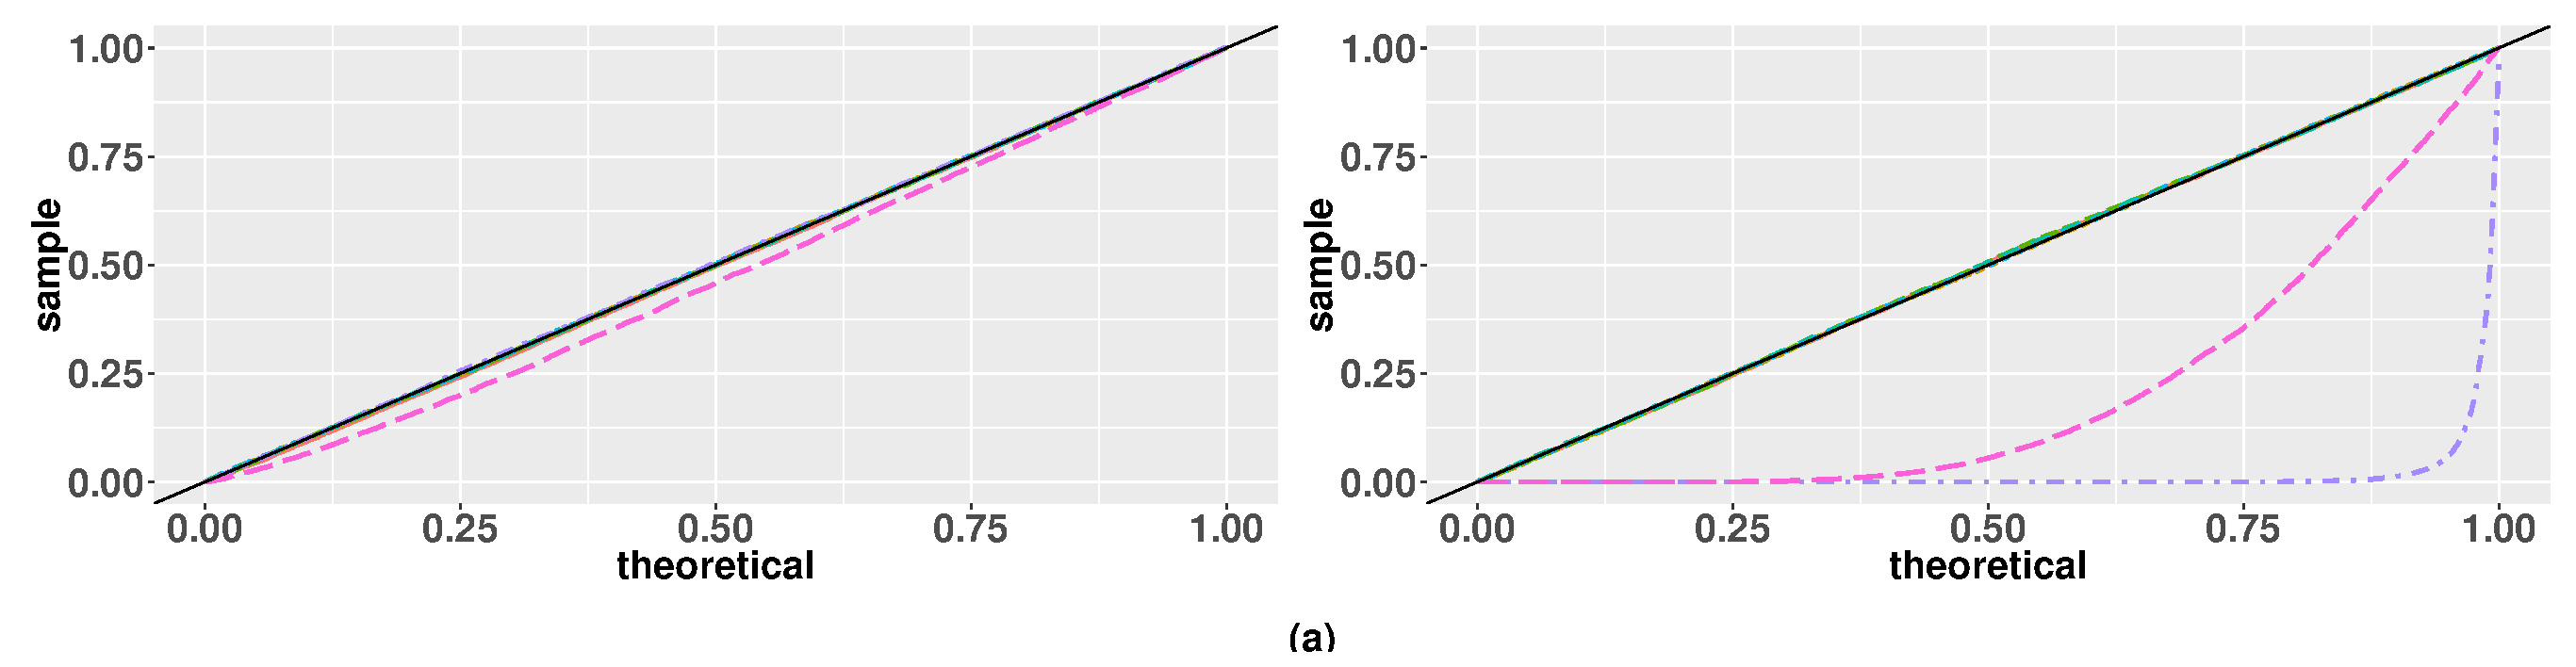
\includegraphics[width=18cm,height=4cm]{Figures/parallel_a.eps}
	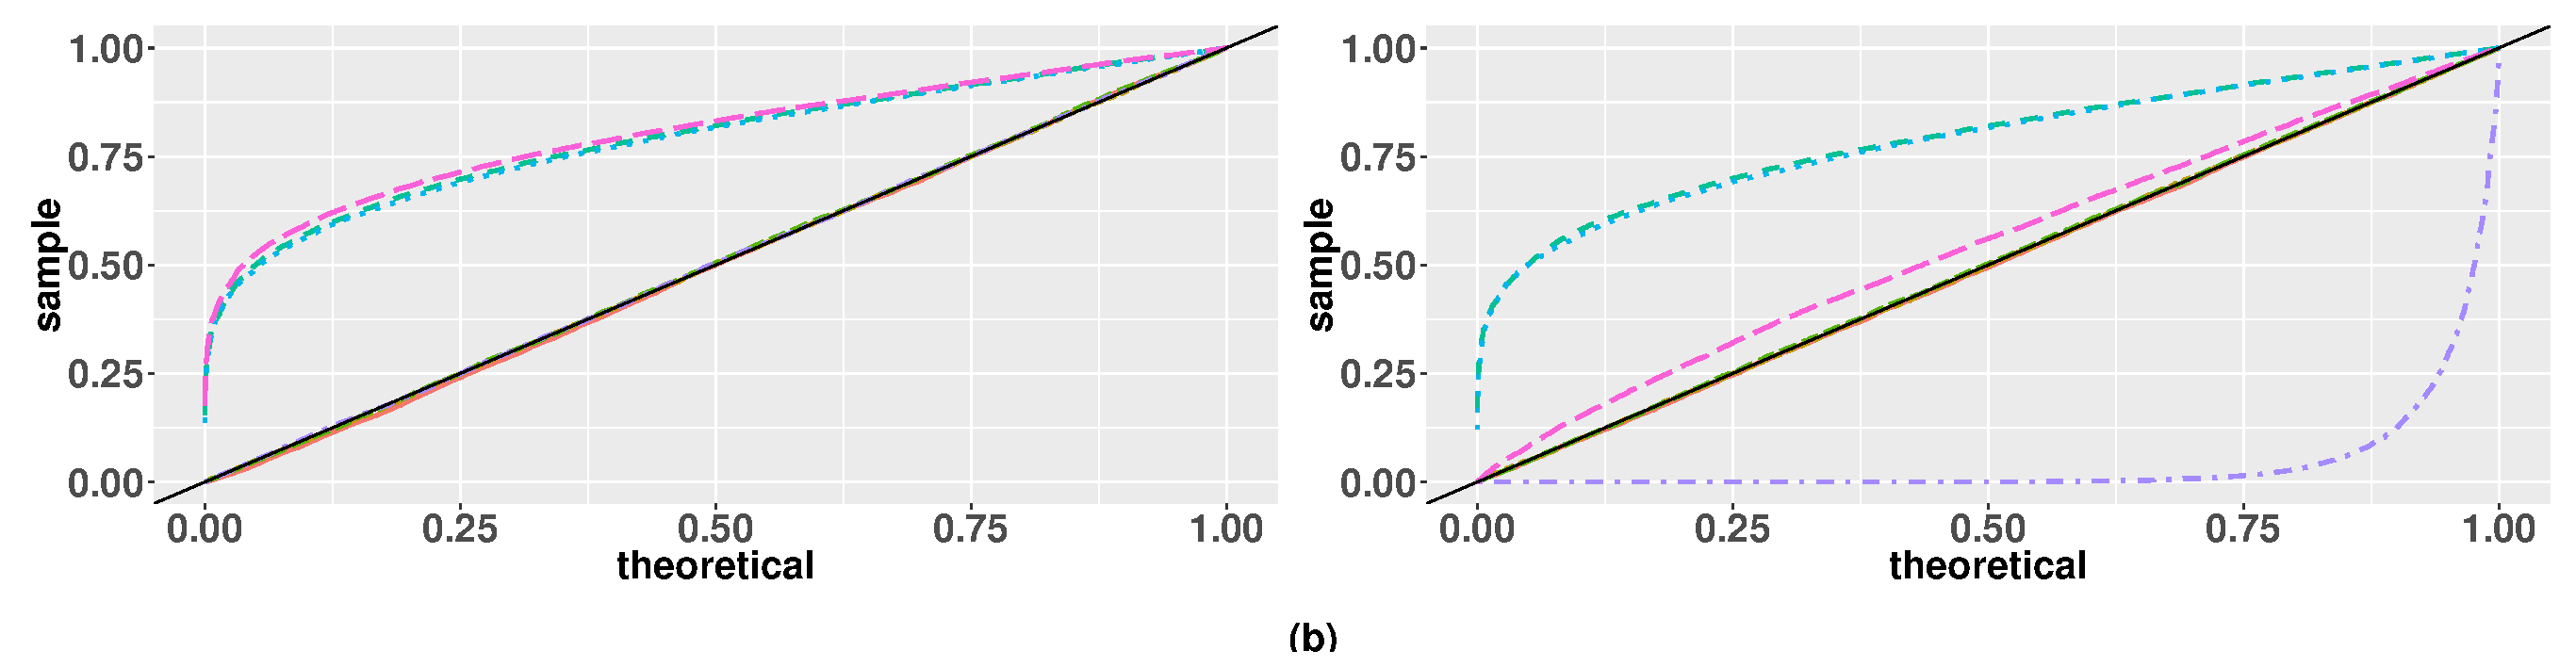
\includegraphics[width=18cm,height=4cm]{Figures/parallel_b.eps}
	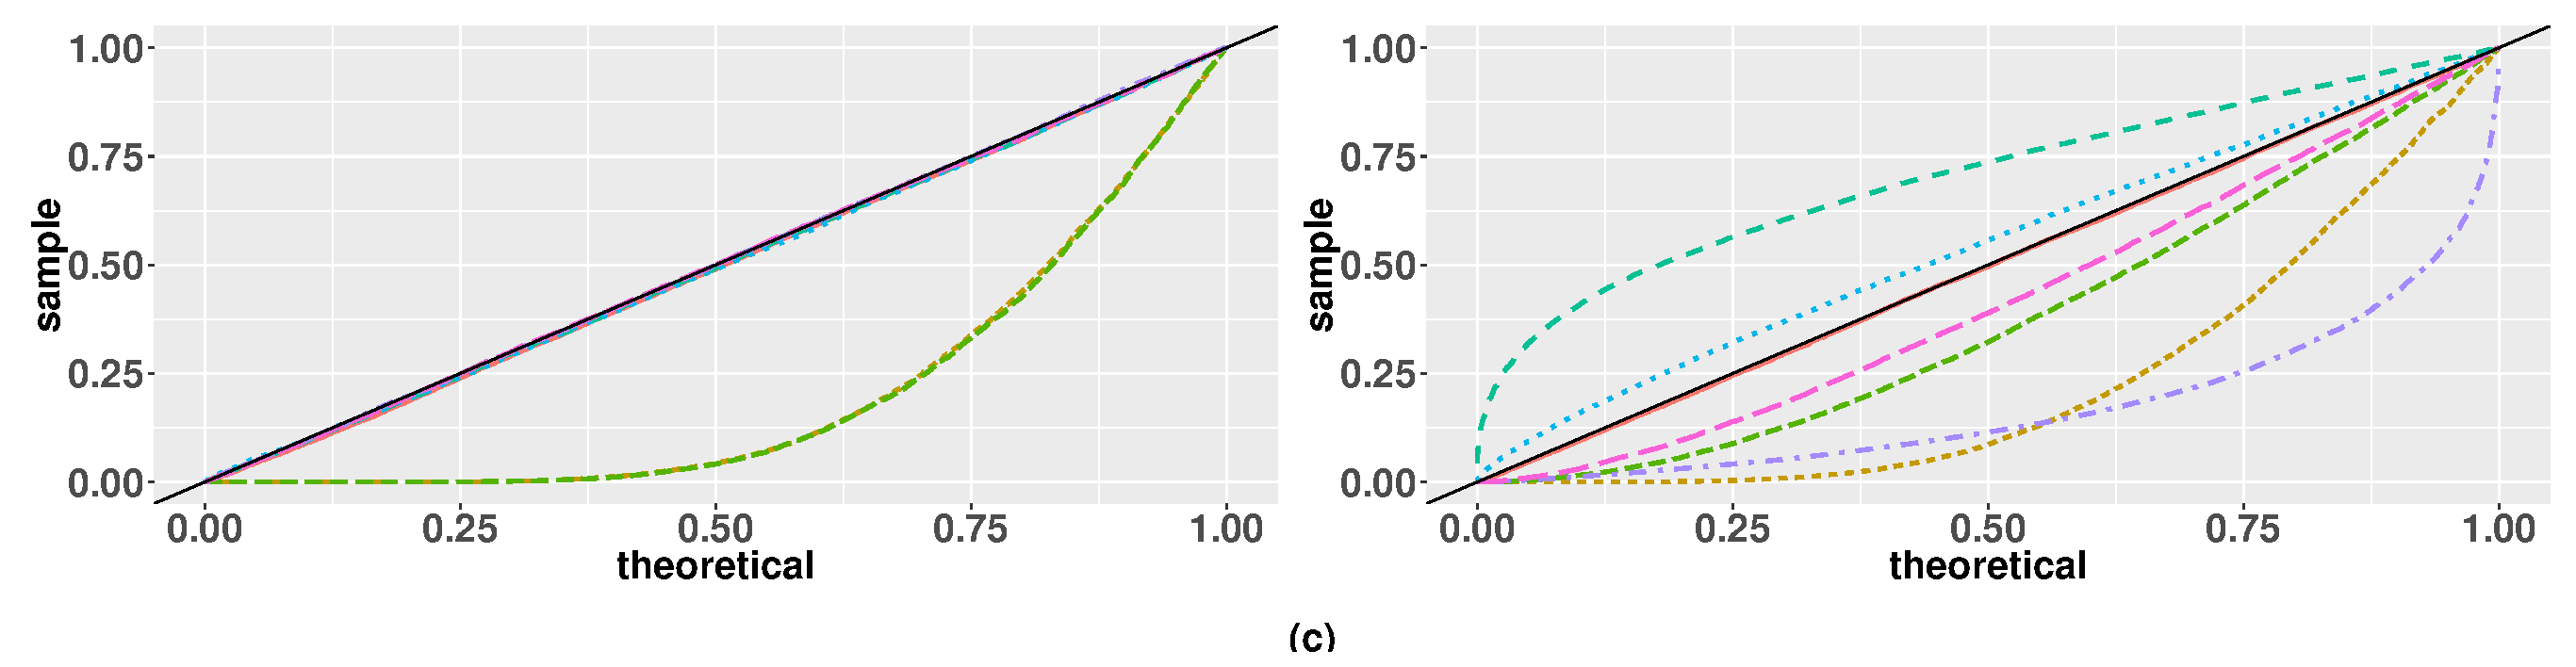
\includegraphics[width=18cm,height=4cm]{Figures/parallel_c.eps}
	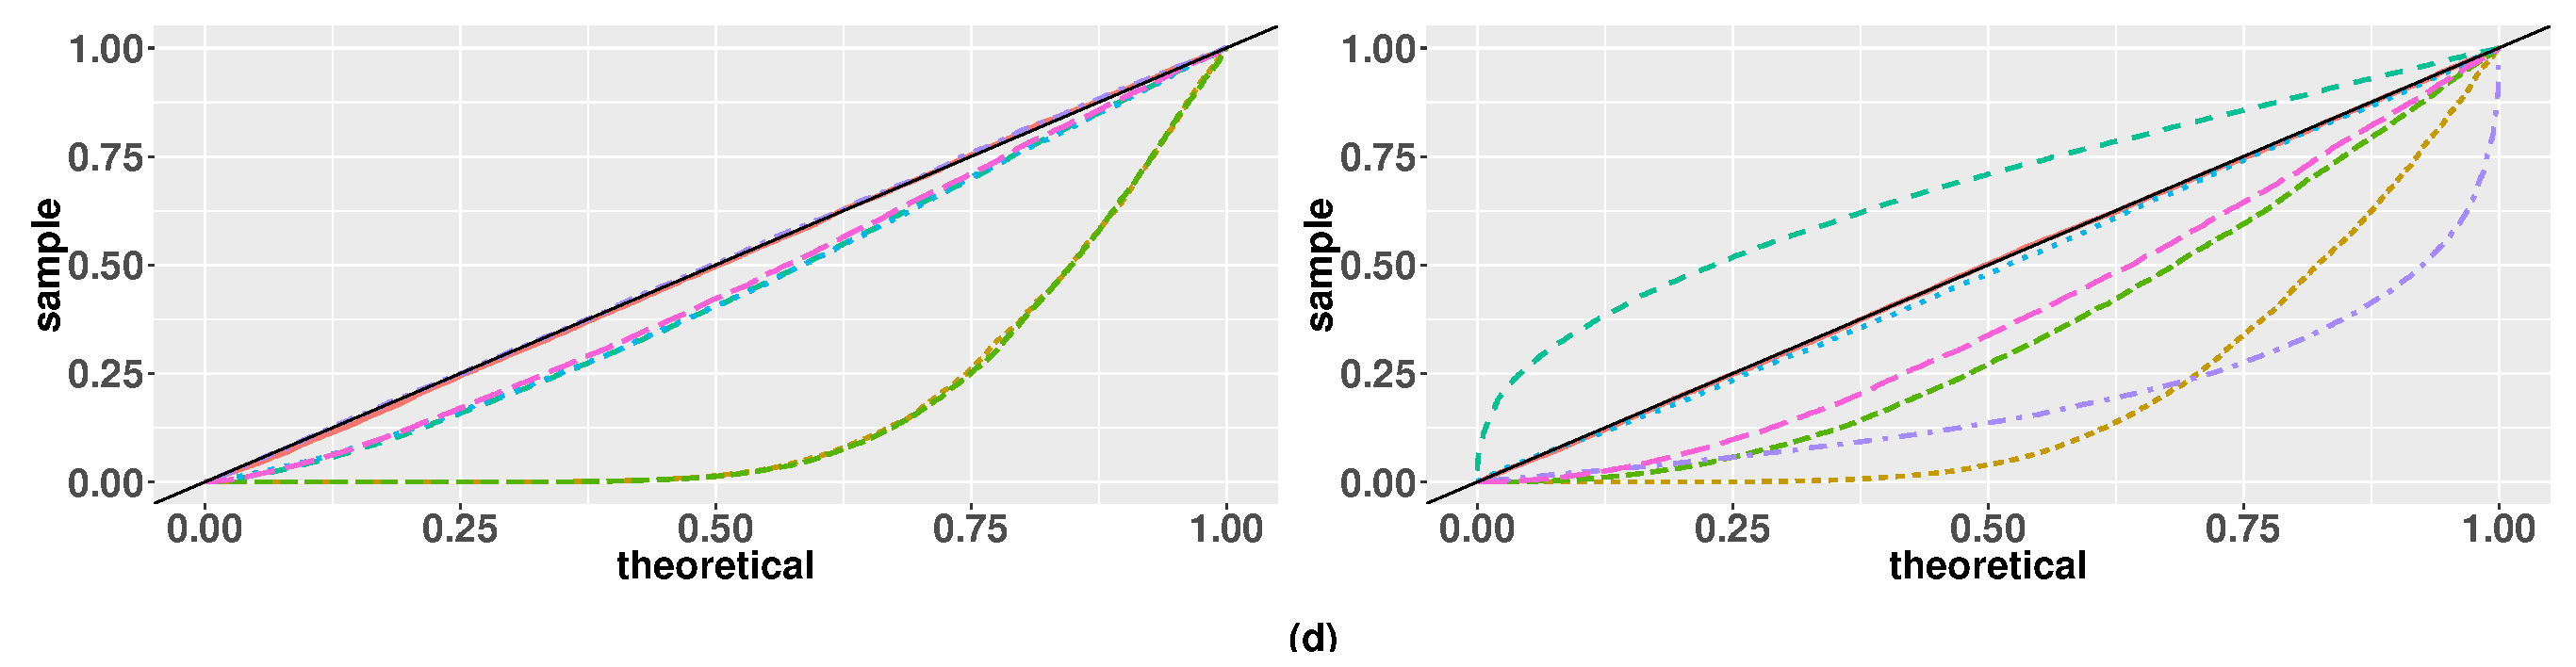
\includegraphics[width=18cm,height=4cm]{Figures/parallel_d.eps}
	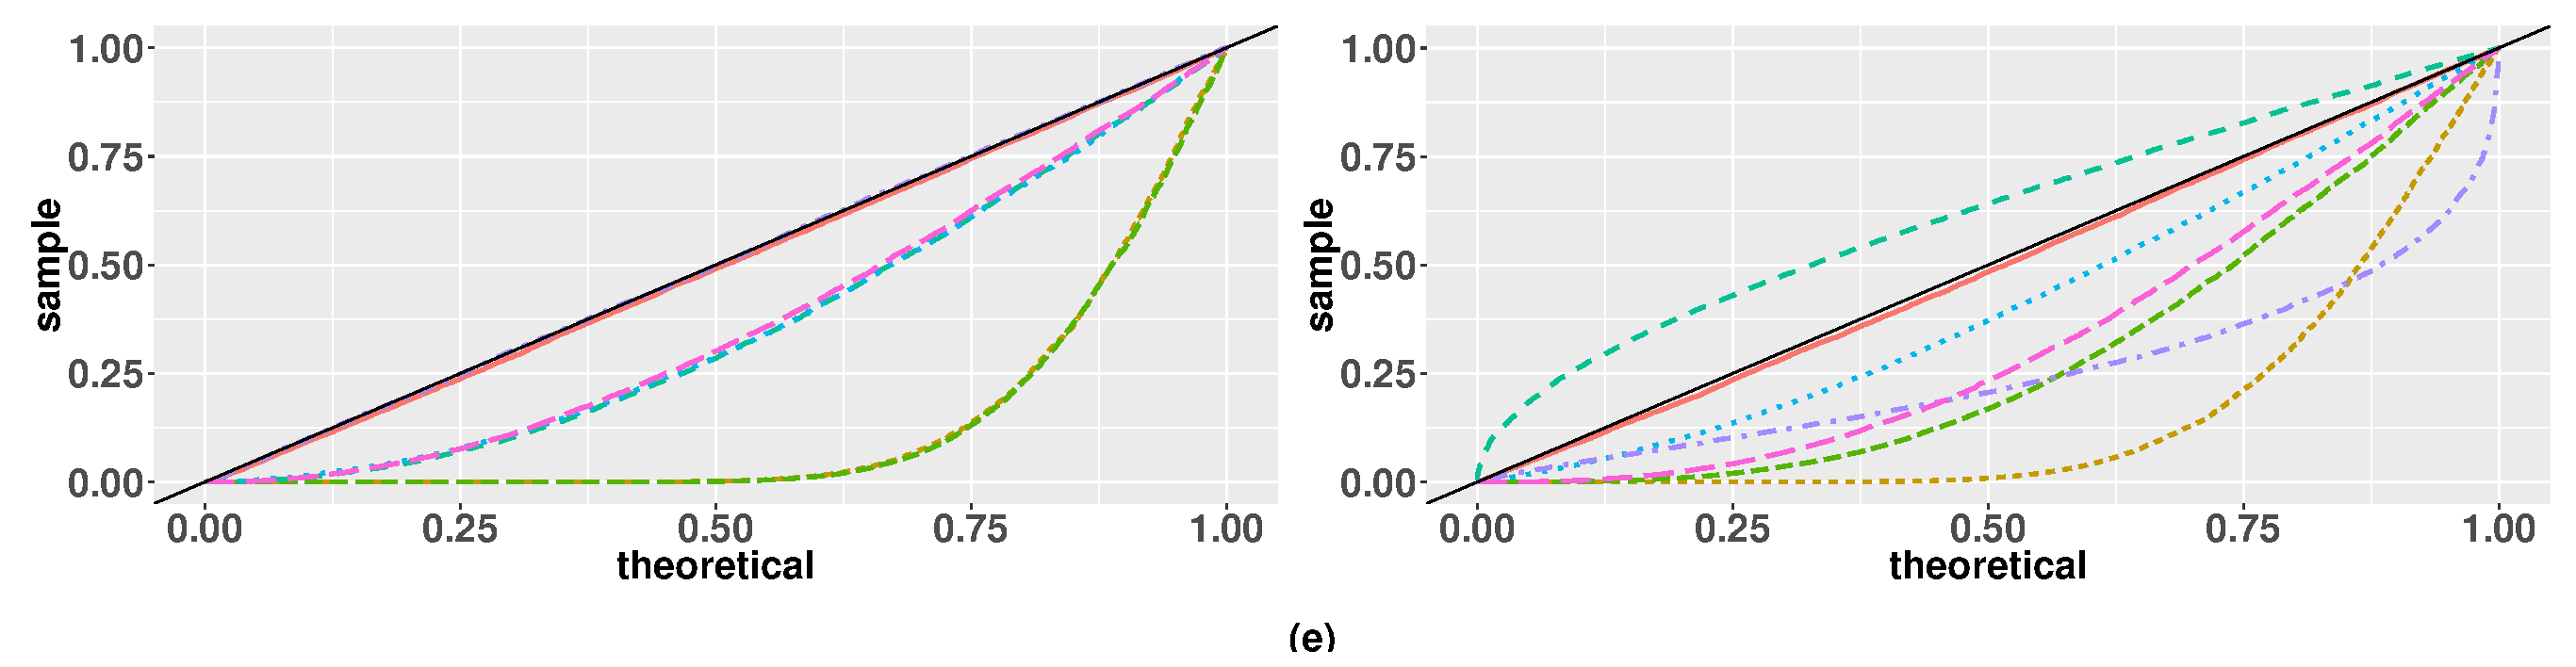
\includegraphics[width=18cm,height=4cm]{Figures/parallel_e.eps}
	%	\includegraphics[width=8cm,height=4cm]{Figures/c_SizePoint1_10PCT.eps}
	%	\includegraphics[width=8cm,height=4cm]{Figures/e_SizePoint1_0PCT.eps}
	%	\includegraphics[width=8cm,height=4cm]{Figures/e_SizePoint1_10PCT.eps}
	%	\includegraphics[width=8cm,height=4cm]{Figures/f_SizePoint1_0PCT.eps}
	%	\includegraphics[width=8cm,height=4cm]{Figures/f_SizePoint1_10PCT.eps}
	\end{center} 
	\caption{Uniform quantile-quantile plots for $p$-values by different methods. Each plot from top to bottom corresponds to correlation structures (\aaCase)-(\fCase), respectively. The left column is for group $A_1$ simulation, and the right column for group $A_2$ simulation (see Table \ref{table:simusetup} for detail). Results are based on \HowmanySimu~simulations.}\label{fig:typeIerror}
\end{figure*} 

	
	\subsection{Power simulation}\label{subsection:power}		 


	
	We compare the power of \OurMethod~to those of the other \HowmanyTest~methods under different correlation structures. Since some of these tests are not well calibrated at the sample size considered (see results in Section \ref{subsection:typeIerror}), we report calibrated power. For calibrated power, the critical value $c(\alpha)$ is chosen so that when the null hypothesis is true, exactly $100\cdot\alpha\%$ of the resulting $p$-values are less than $c(\alpha)$; that is, $c(\alpha)$ is  the $\alpha$ quantile of null distribution of $p$-values, where the null distribution is generated from simulation. Calibrated power allows a more fair comparison among tests, as tests that are too conservative under the null hypothesis will have greater power due to the tendency to produce small $p$-values, yet this apparent power does not truly distinguish between the null and the alternative.  
	
	Table \ref{table:power} summarizes the calibrated power for the two groups of simulations (i.e., $A_1$ and $A_2$ in Table \ref{table:simusetup}). We only report the results for correlation structure (\aaCase) where genes are simulated to be independent. %(for power comparisons under the other four correlation structures, see online supplementary materials...). %In Table \ref{table:power} we set the DE size $\delta$ to be 0.05 and simulated data in the way that genes in the background set are not DE (i.e., $p_b=0$). 
	For $A_1$ simulations, GSEA has the highest, and rank based methods MRSGE and \CMR~have the lowest, calibrated power across all four alternative scenarios (the data for $S_4$ not shown). \CMT~and \OurMethod~have no systematic difference in the calibrated power. % Furthermore, when the DE probability is $10\%$ or higher (i.e., the case of  $S_2$-$S_4$), both \CMT~and \OurMethod~have comparable calibrated power to that of GSEA and \gent. In group $A_2$, \gent~continues to achieve the highest calibrated power while GSEA shows virtually no power. \CMT~and \OurMethod~still have indistinguishable calibrated power and both are better than MRSGE and \CMR.
	 In group $A_2$ simulations, GSEA shows virtually no power. \OurMethod, \CMT, \gent~and QuSAGE have indistinguishable calibrated power and are among the best. 	

	
% \begin{table*}
%	\centering
%	\caption{Recalibrated power (standard error) for different methods. The powers are summarized under three alternatives $S_1$-$S_3$ in each of the group $A_1$ and $A_2$ simulations (see Table \ref{table:simusetup} for detail). Results are based on \HowmanySimu~simulations. }\label{table:power}
%	\begin{tabular}{rcccc c cccc}
%		\hline\hline
%		Method	& \multicolumn{4}{c}{Group $A_1$} &  & \multicolumn{4}{c}{Group $A_2$} \\
%		\cline{2-5}   \cline{7-10}
%		& $S_1$ & $S_2$ & $S_3$	&$S_4$ & & $S_1$ & $S_2$ & $S_3$ &$S_4$ \\
%		\cline{2-5}   \cline{7-10}
%		\OurMethod & 0.335(0.015) & 0.765(0.013) & 0.959(0.006) & 0.996(0.002) & & 0.199(0.013) & 0.538(0.016) & 0.836(0.012) & 0.959(0.006)\\ 
%		\genr & 0.129(0.011) & 0.344(0.015) & 0.609(0.015) & 0.839(0.012) &  & 0.121(0.010) & 0.334(0.015) & 0.626(0.015) & 0.866(0.011) \\
%		\gent & 0.350(0.015) & 0.778(0.013) & 0.961(0.006) & 0.995(0.002)& & 0.201(0.013) & 0.534(0.016) & 0.846(0.011) & 0.961(0.006) \\ 
%		CAMERA1 & 0.347(0.015) & 0.767(0.013) & 0.960(0.006) & 0.995(0.002)&  & 0.197(0.013) & 0.531(0.016) & 0.837(0.012) & 0.960(0.006) \\ 
%		CAMERA2 & 0.119(0.010) & 0.331(0.015) & 0.602(0.015) & 0.834(0.012) & & 0.118(0.010) & 0.329(0.015) & 0.619(0.015) & 0.859(0.011)\\
%		GSEA & 0.486(0.016) & 0.891(0.010) & 0.996(0.002) & 0.998(0.001) & & 0.000(0.000) & 0.000(0.000) & 0.000(0.000) & 0.000(0.000) \\ 
%		QuSAGE & 0.387(0.015) & 0.804(0.013) & 0.977(0.005) & 0.996(0.002)  & & 0.197(0.013) & 0.536(0.016) & 0.846(0.011) & 0.960(0.006) \\ 
%		\hline\hline
%	\end{tabular}
%\end{table*}

	% latex table generated in R 3.2.3 by xtable 1.8-0 package
	% Sat Mar 26 11:41:31 2016
	\begin{table*}[ht]
			\centering
			\caption{Recalibrated power (standard error) for different methods. The powers are summarized under three alternatives $S_1$-$S_3$ in each of the group $A_1$ and $A_2$ simulations (see Table \ref{table:simusetup} for detail). Results are based on \HowmanySimu~simulations. }\label{table:power}
		\begin{tabular}{cl M{2.5cm}M{2.5cm}M{2.5cm}M{2.5cm}}
			\hline\hline
		Group & Method	& $S_1$ & $S_2$ & $S_3$	&$S_4$  \\ 
			\hline
		\multirow{7}{*}{$A_1$} &	MEQLEA & 0.335(0.015) & 0.765(0.013) & 0.959(0.006) & 0.996(0.002) \\ 
		&	\genr & 0.129(0.011) & 0.344(0.015) & 0.609(0.015) & 0.839(0.012) \\ 
		&	\gent & 0.350(0.015) & 0.778(0.013) & 0.961(0.006) & 0.995(0.002) \\ 
		&	\CMT & 0.347(0.015) & 0.767(0.013) & 0.960(0.006) & 0.995(0.002) \\ 
		&	\CMR & 0.119(0.010) & 0.331(0.015) & 0.602(0.015) & 0.834(0.012) \\ 
		&	GSEA & 0.486(0.016) & 0.891(0.010) & 0.996(0.002) & 0.998(0.001) \\ 
		&	QuSAGE & 0.387(0.015) & 0.804(0.013) & 0.977(0.005) & 0.996(0.002) \\ 
				\hline	
		\multirow{7}{*}{$A_2$} &	MEQLEA & 0.199(0.013) & 0.538(0.016) & 0.836(0.012) & 0.959(0.006) \\ 
		&		\genr & 0.121(0.010) & 0.334(0.015) & 0.626(0.015) & 0.866(0.011) \\ 
		&		\gent & 0.201(0.013) & 0.534(0.016) & 0.846(0.011) & 0.961(0.006) \\ 
		&		\CMT & 0.197(0.013) & 0.531(0.016) & 0.837(0.012) & 0.960(0.006) \\ 
		&		\CMR & 0.118(0.010) & 0.329(0.015) & 0.619(0.015) & 0.859(0.011) \\ 
		&		GSEA & 0.000(0.000) & 0.000(0.000) & 0.000(0.000) & 0.000(0.000) \\ 
		&		QuSAGE & 0.197(0.013) & 0.536(0.016) & 0.846(0.011) & 0.960(0.006) \\ 
				\hline\hline
		\end{tabular}
	\end{table*}
	
	
	
	Figure \ref{fig:power} shows for \OurMethod, the variations in power according to different correlation structures across four alternative scenarios $S_1$-$S_4$. For each correlation structure and each alternative, we report the power (without recalibration) at a significance level of 0.05. The top is the power for group $A_1$, and the bottom for group $A_2$.  The powers for case (\aaCase) and (\cCase) are very similar, and are among the highest under each of the four alternatives. It's not surprising because they correspond to the simplest correlation structures: gene expression values in (\aaCase) are simulated to be independent and in (\cCase) are simulated to have the same correlation 0.1. As the correlation structure becomes more complex, from (\aCase) to (\eCase) then to (\fCase), the power decreases under every alternative scenario. The power under correlation structure (\fCase) is the lowest for both $A_1$ and $A_2$ simulations.% We also note that the power decreases when DE genes are present in the background set as compared to the case where there are no DE genes in the background set. (We might need the same DE size to illustrate this point.)
	
\begin{figure}
	\begin{center}
		\includegraphics[width=8.5cm,height=5cm]{Figures/powerBack0pct.eps}
		\includegraphics[width=8.5cm,height=5cm]{Figures/powerBack10pct.eps}
	\end{center} 
		\caption{Power for \OurMethod~under correlation structures (\aaCase)-(\fCase) of Section \ref{subsection:simulation}. The top corresponds to group $A_1$ simulations, and the bottom to group $A_2$ simulations (see Table \ref{table:simusetup}). The error bars are the $95\%$ CIs based on \HowmanySimu~simulations. }\label{fig:power}
\end{figure} 
	
	\subsection{Real Data}\label{section:realdata}
	We applied \OurMethod~to two example data sets, and compared the enriched gene sets to those obtained by GSEA and by \CMT. In both examples, \OurMethod~were able to identify more gene sets as enriched. Our results lend credence to previous studies in finding potential gene sets correlated with Huntington's disease and those correlated with chromosome Y and Y bands in lymphoblastoid cells.  
	
	\subsubsection{Huntington's Disease Data}
	We examined the Huntington's Disease (HD) RNA-Sequencing (RNA-Seq) data \citep{labadorf2015rna}  to identify which gene sets are enriched among DE genes in HD. The mRNA expression profiles in human prefrontal cortex were obtained from 20 Huntington's Disease samples and 49 neurologically normal controls.  Expression values were normalized and filtered as described in the methods section of \cite{labadorf2015rna}.
	The data, containing $28,087$ genes, is available as a series GSE64810 in the GEO database (\url{http://www.ncbi.nlm.nih.gov/geo/}). We performed enrichment analysis using the MsigDB \citep{subramanian2005gene} C2 Canonical Pathways gene sets (February 5, 2016, data last accessed). The C2 Canonical Pathway gene sets have a collection of 1330 gene sets, with an average set size of 50 (the set sizes range from 3 to 1028, and the median is 29). Since the genes in C2 are named by HGNC symbols and by ensembl IDs in the HD expression data set, we converted the ensembl IDs in the expression data into HGNC symbols using \textit{BioMart} (\url{http://uswest.ensembl.org/biomart/martview/}). We retained $26,941$ genes that have corresponding HGNC symbols. For \OurMethod, we standardized the data in the way as described in Section....
	
	
	We used three test procedures (\OurMethod, GSEA and \CMT) to run enrichment analysis for the entire C2 Canonical Pathway gene sets, and compared the three tests in terms of resulting enriched gene sets. \OurMethod~found 176 out of 1330 gene sets to be enriched using the Benjamini-Hochberg (BH) procedure at a false discovery rate (FDR) of 0.05 (for multiple hypothesis testing, unless specified otherwise, all $p$-values in Section \ref{section:realdata} were adjusted by BH procedure). GSEA found 9 enriched gene sets---8 of them were also among the 176 gene sets we identified (the one that was not significant according to \OurMethod~had a $p$-value of 0.008 and FDR 0.057). \CMT~found no enriched gene sets. In Figure \ref{fig:HDdatap} we present pairwise $p$-value plots for \OurMethod, GSEA and \CMT. When plotted against $p$-values of GSEA, for \OurMethod, smaller $p$-values (e.g., less than 0.1) are more likely to cluster---as compared to larger $p$-values; that is, \OurMethod~produces more small $p$-values than GSEA does while \OurMethod~and GSEA do not differ much in producing larger $p$-values. The $p$-values of \CMT~are overwhelmingly larger than their counterparts of \OurMethod, even if $p$-values of the two methods are highly correlated (Pearson's correlation is 0.96). This is consistent with our earlier simulation (see results in Section \ref{subsection:typeIerror}) that \CMT~could be too conservative. There is no systematic difference in $p$-values of GSEA and those of \CMT. 
\begin{figure}
	\begin{center}
		\includegraphics[width=8cm,height=5cm]{Figures/P_GSEA.eps}
		\includegraphics[width=8cm,height=5cm]{Figures/P_Camera.eps}
		\includegraphics[width=8cm,height=5cm]{Figures/P_GSEA_CAMERA.eps}
	\end{center} 
		\caption{Pairwise comparisons of $p$-values for \OurMethod, GSEA, and \CMT. The $p$-values are reported from enrichment test of each gene set in the C2 Canonical Pathway gene sets. }\label{fig:HDdatap}
\end{figure} 
	
%	\begin{figure}
%		\begin{center}
%			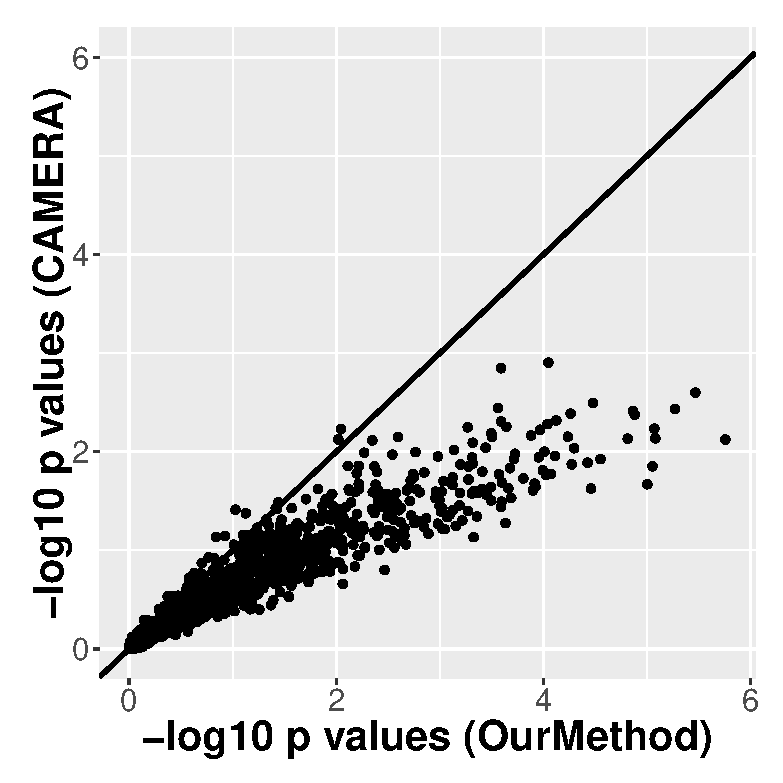
\includegraphics[width=5.5cm,height=5cm]{Figures/log10P_Camera.eps}
%			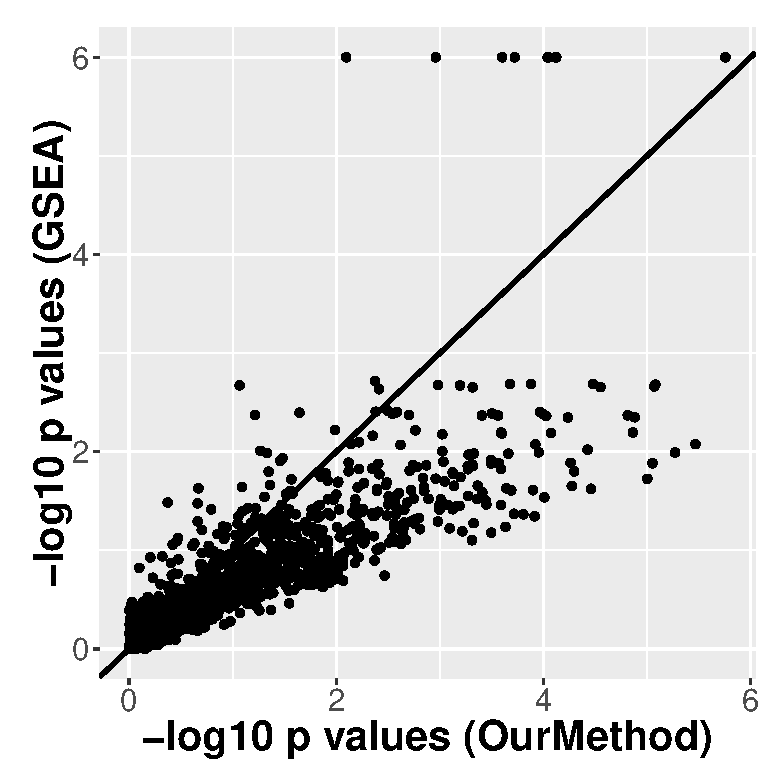
\includegraphics[width=5.5cm,height=5cm]{Figures/log10P_GSEA.eps}
%			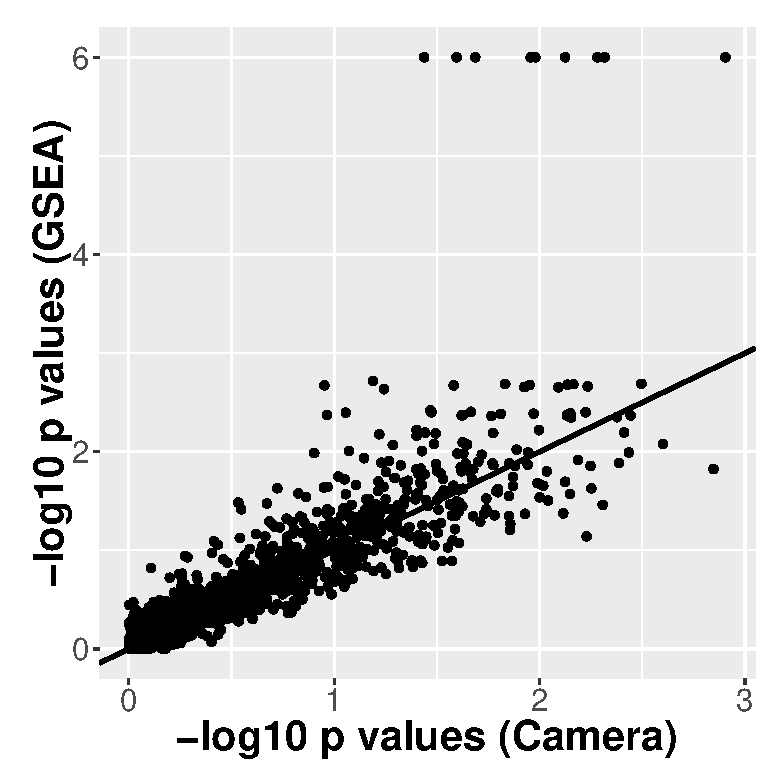
\includegraphics[width=5.5cm,height=5cm]{Figures/log10P_GSEA_CAMERA.eps}
%		\end{center} 
%				\caption{raw p value plots for different methods, -log10(p  + 1e-6)}\label{fig:HDdatalog10p}
%	\end{figure} 
	
	We report the top 30 enriched gene sets in Table \ref{table:top30}. Five enriched gene sets identified by GSEA are also present (noted by ``$\ast$" in the table). Originally, \cite{labadorf2015rna} used the same HD data set to conduct enrichment analysis using topGo \citep{alexa2010topgo}. They found that the enriched gene sets they identified show a clear immune response and inflammation-related pattern, including ``REACTOME INNATE IMMUNE SYSTEM, PID IL4 2PATHWAY", and ``PID NFKAPPAB CANONICAL PATHWAY". These three gene sets rank 6,10 and 2 respectively in Table \ref{table:top30}.
	
	Many of our enriched gene sets have been shown to be closely related to HD pathogenesis. For example, the top enriched gene set by \OurMethod,``PID SMAD2 3NUCLEAR PATHWAY" (see Table \ref{table:top30}), is responsible for regulation of nuclear SMAD2/3 signaling. \cite{katsuno2010disrupted} showed that nuclear SMAD2/3 are related to polyglutamine disease, which includes HD. The second enriched gene set, ``PID NFKAPPAB CANONICAL PATHWAY", is a canonical NF-kappaB pathway, and its dysregulation causes HD immune dysfunction \citep{trager2014htt}. Also, \cite{marcora2010huntington} found that reduced transport of NF-kappaB out of dendritic spines and its activity in neuronal nuclei may contribute to the etiology of HD. 
	%HD mutation can reduce the transport of NF-kappaB out of dendritic spines and its activity in neuronal nuclei and this reduction may contribute to the etiology of HD. 
	Another gene set, ``REACTOME INNATE IMMUNE SYSTEM", contributes to HD pathogenesis \citep{trager2014htt, labadorf2015rna}. %\cite{diamanti2013whole} showed that ``REACTOME TRANSCRIPTIONAL ACTIVITY OF SMAD2 SMAD3 SMAD4 HETEROTRIMER", a gene set involved in transcriptional activity of SMAD2/SMAD3:SMAD4 heterotrimer, is also enriched in their microarray study of HD pathology from blood samples of R6/2 at manifest stage and wild type littermate mice. 
	For AKT signaling pathway, ``BIOCARTA AKT PATHWAY", \cite{humbert2002igf} demonstrated that huntingtin is a substrate of AKT and that phosphorylation of huntingtin by AKT is crucial to mediate the neuroprotective effects of IGF-1. They also showed that AKT is altered in Huntington’s disease patients.  
	\cite{chiang2010modulation} demonstrated that the systematic downregulation of PPAR$\gamma$, related to ``BIOCARTA PPARA PATHWAY", seems to play a critical role in the dysregulation of energy homeostasis observed in HD, and that PPAR$\gamma$ is a potential therapeutic target for this disease. For ``REACTOME SIGNALING BY TGF BETA RECEPTOR COMPLEX",  \cite{kandasamy2011transforming} demonstrated that TGF-beta1 signaling appears to be a crucial modulator of neurogenesis in HD pathology and it can be a promising target for endogenous cell-based regenerative therapy. 
	For ``PID P53 DOWNSTREAM PATHWAY", \cite{ghose2011regulation} showed the likely involvement of NFkB (RelA), p53 and miRNAs in the regulation of cell death in HD pathogenesis. 
	
	
\begin{table*}[!ht]
	%	\label{table:gender} 
	\centering 
		\caption{Top 30 enriched gene sets using \OurMethod~for HD data. Gene sets are ranked by their associated $p$-values. FDR is the adjusted $p$-value using Benjamini-Hochberg (BH) procedure. }
	\begin{tabular}{p{3in}M{0.5cm}M{0.7cm}M{0.7cm}M{0.7cm}M{1.5cm}M{1.5cm}M{0.8cm}} 
		\hline
		\hline
		Gene Set & Size & $\rho_1$ & $\rho_2$ & $\rho_3$ & $p$-value & FDR & \\ 
		\hline
		PID SMAD2 3NUCLEAR PATHWAY & 79 & 0.071 & 0.011 & 0.017 & 7.5E-07 & 9.9E-04 & $\ast$, $\ast\ast$ \\ 
		PID NFKAPPAB CANONICAL PATHWAY & 22 & 0.124 & 0.011 & 0.020 & 2.4E-06 & 1.6E-03 & $\ast\ast$ \\ 
		REACTOME YAP1 AND WWTR1 TAZ STIMULATED GENE EXPRESSION & 23 & 0.130 & 0.011 & 0.018 & 4.4E-06 & 1.7E-03 & $\ast\ast$ \\ 
		REACTOME SIGNALING BY TGF BETA RECEPTOR COMPLEX & 60 & 0.045 & 0.011 & 0.015 & 7.3E-06 & 1.7E-03 & $\ast\ast$ \\ 
		BIOCARTA NTHI PATHWAY & 23 & 0.124 & 0.011 & 0.024 & 7.5E-06 & 1.7E-03 &  \\ 
		REACTOME INNATE IMMUNE SYSTEM & 209 & 0.048 & 0.011 & 0.010 & 7.8E-06 & 1.7E-03 & $\ast\ast$ \\ 
		KEGG PATHWAYS IN CANCER & 311 & 0.029 & 0.011 & 0.010 & 8.9E-06 & 1.7E-03 &  \\ 
		REACTOME DOWNSTREAM TCR SIGNALING & 31 & 0.095 & 0.011 & 0.013 & 1.2E-05 & 1.9E-03 & $\ast\ast$ \\ 
		KEGG NOD LIKE RECEPTOR SIGNALING PATHWAY & 55 & 0.054 & 0.011 & 0.010 & 1.3E-05 & 1.9E-03 & $\ast\ast$ \\ 
		PID IL4 2PATHWAY & 59 & 0.086 & 0.011 & 0.012 & 1.4E-05 & 1.9E-03 &  $\ast\ast$\\ 
		KEGG TGF BETA SIGNALING PATHWAY & 82 & 0.062 & 0.011 & 0.013 & 2.7E-05 & 3.3E-03 & $\ast\ast$ \\ 
		BIOCARTA 41BB PATHWAY & 14 & 0.095 & 0.011 & 0.023 & 3.2E-05 & 3.4E-03 &  \\ 
		PID P53 DOWNSTREAM PATHWAY & 131 & 0.052 & 0.011 & 0.013 & 3.4E-05 & 3.4E-03 & $\ast\ast$ \\ 
		REACTOME TCR SIGNALING & 48 & 0.098 & 0.011 & 0.016 & 3.6E-05 & 3.5E-03 & $\ast\ast$ \\ 
		REACTOME ACTIVATED TLR4 SIGNALLING & 87 & 0.027 & 0.011 & 0.010 & 4.9E-05 & 4.2E-03 & $\ast\ast$ \\ 
		REACTOME TOLL RECEPTOR CASCADES & 110 & 0.038 & 0.011 & 0.010 & 5.2E-05 & 4.2E-03 & $\ast\ast$ \\ 
		REACTOME TRANSCRIPTIONAL REGULATION OF WHITE ADIPOCYTE DIFFERENTIATION & 69 & 0.015 & 0.011 & 0.010 & 5.4E-05 & 4.2E-03 &  \\ 
		BIOCARTA TID PATHWAY & 18 & 0.125 & 0.011 & 0.017 & 5.7E-05 & 4.2E-03 & $\ast\ast$ \\ 
		BIOCARTA ALK PATHWAY & 34 & 0.064 & 0.011 & 0.011 & 7.4E-05 & 5.1E-03 & $\ast$ \\ 
		REACTOME SMAD2 SMAD3 SMAD4 HETEROTRIMER REGULATES TRANSCRIPTION & 25 & 0.102 & 0.011 & 0.021 & 7.6E-05 & 5.1E-03 & $\ast$ \\ 
		REACTOME TRANSCRIPTIONAL ACTIVITY OF SMAD2 SMAD3 SMAD4 HETEROTRIMER & 36 & 0.079 & 0.011 & 0.021 & 8.3E-05 & 5.1E-03 &  \\ 
		BIOCARTA AKT PATHWAY & 20 & 0.023 & 0.011 & 0.010 & 8.8E-05 & 5.1E-03 & $\ast$ \\ 
		ST TUMOR NECROSIS FACTOR PATHWAY & 28 & 0.039 & 0.011 & 0.016 & 9.0E-05 & 5.1E-03 & $\ast$ \\ 
		PID ANGIOPOIETIN RECEPTOR PATHWAY & 50 & 0.082 & 0.011 & 0.013 & 9.3E-05 & 5.1E-03 & $\ast\ast$ \\ 
		KEGG P53 SIGNALING PATHWAY & 65 & 0.037 & 0.011 & 0.007 & 9.7E-05 & 5.1E-03 &  \\ 
		KEGG APOPTOSIS & 82 & 0.041 & 0.011 & 0.009 & 1.0E-04 & 5.1E-03 &  \\ 
		BIOCARTA PPARA PATHWAY & 53 & 0.026 & 0.011 & 0.008 & 1.1E-04 & 5.2E-03 &  \\ 
		REACTOME MYD88 MAL CASCADE INITIATED ON PLASMA MEMBRANE & 78 & 0.026 & 0.011 & 0.010 & 1.1E-04 & 5.2E-03 &  $\ast\ast$\\ 
		PID BCR 5PATHWAY & 64 & 0.064 & 0.011 & 0.016 & 1.2E-04 & 5.3E-03 &  \\ 
		PID HIF1 TFPATHWAY & 64 & 0.067 & 0.011 & 0.011 & 1.2E-04 & 5.3E-03 &  \\ 
		\hline\hline
		\multicolumn{7}{l}{$\rho_1$: average sample correlation between genes in the test set. }	 \\	
		\multicolumn{7}{l}{$\rho_2$: average sample correlation between genes in the background set. }	 \\	
		\multicolumn{7}{l}{$\rho_3$: average sample correlation between two genes, one from the test set and the other from the background set. }	 \\	
		\multicolumn{7}{l}{ ~~$\ast$: enriched gene sets identified by GSEA.}	 \\	
		\multicolumn{7}{l}{$\ast\ast$: enriched gene sets identified by \genr.}	 \\	
				
		%	\hline\hline
	\end{tabular}
\label{table:top30}
\end{table*}

	
	
	
%	
	
	
	\subsubsection{Male vs Female Lymphoblastoid Cells Data}
	We analyzed the mRNA expression profiles from lymphoblastoid cell lines derived from 17 females and 15 males. \cite{subramanian2005gene} examined this data set with their GSEA method, testing the enrichment of the  cytogenetic gene sets (C1). C1 includes 24 sets, one for each of the 24 human chromosomes, and 295 sets corresponding to cytogenetic bands. For the comparison ``\text{male} VS \text{female}", they expected to find gene sets on chromosome Y, not on chromosome X. We run enrichment analysis with three tests (\OurMethod, GSEA and \CMT). In Table \ref{table:gender}, we summarized all the gene sets with nominal $p$-value $\leq 0.01$ in at least one test. Three gene sets, one from chromosome Y and two Y bands, were found to be enriched by all three tests at FDR level 0.05. Interestingly, \OurMethod~identified another Y band, chrYp22, as enriched. In fact, the four gene sets called significant by \OurMethod~are the only four containing at least 3 genes in C1 and corresponding to chromosome Y or Y bands. \OurMethod~ did not produce small $p$-value ($\leq 0.01$ ) for the remaining three gene sets in Table \ref{table:gender}, which was just as expected in that study.
	
\begin{table*}[!th]
	%	\label{table:gender} 
	\centering
	\caption{Summary of gene sets for lymphoblastoid cells data. Reported are gene sets with $p$-value $\leq 0.01$ for at least one of the \OurMethod, GSEA, and \CMT~methods. The FDR is the adjusted $p$-value using Benjamini-Hochberg (BH) procedure.}
	\begin{tabular}{lM{1.5cm}M{1.5cm}M{1.5cm} c M{1.5cm}M{1.5cm} c M{1.5cm}M{1.5cm}} \hline\hline 
		& &  \multicolumn{2}{c}{\OurMethod} & & \multicolumn{2}{c}{GSEA}	& & \multicolumn{2}{c}{\CMT} \\	
		\cline{3-4}  \cline{6-7} \cline{9-10}
		Gene set & Size & $p$-value & FDR & & $p$-value & FDR & &$p$-value & FDR \\ 
		\hline
		chrY & 40 & $<0.001$ & $<0.001$ & &$<0.001$ & $<0.001$ & & $<0.001$ & 0.002 \\ 
		chrYq11 & 16 & $<0.001$ & $<0.001$& & $<0.001$ & $<0.001$ & & $<0.001$ & $<0.001$ \\ 
		chrYp11 & 18 & $<0.001$ & $<0.001$ & & $<0.001$ & $<0.001$& & $<0.001$ & 0.028 \\ 
		chrYp22 & 8 & $<0.001$ & 0.036& & 0.012 & 0.503 & & 0.010 & 0.762 \\ 
		chr7p11 & 8 & 0.049 & 0.835 & & 0.006 & 0.352 & & 0.101 & 0.998 \\ 
		chr11p12 & 5 & 0.065 & 0.835& & 0.008 & 0.388 & & 0.115 & 0.998 \\ 
		chrXp22 & 76 & 0.072 & 0.835& & 0.004 & 0.295 & & 0.581 & 0.998 \\  
		\hline\hline
	\end{tabular}
	\label{table:gender}
\end{table*}
	
	\section{Conclusion and Discussion}\label{section:conclusion}
	
	(Conclusion) \OurMethod~is a mixed effects quasi-likelihood model for competitive gene set test. It effectively adjusts for completely unknown, unstructured correlations among the genes. It uses a score test approach and allows for analytical assessment of $p$-values. Compared to existing approaches, \OurMethod~controls type I error correctly and maintains good power under different correlation structures.  
	
	
	(What we proposed) Under competitive gene set test framework, a number of methods have been proposed to account for correlation among genes. One approach is to evaluate the set-level statistic by permuting sample labels to generate the null distribution, as adopted by the widely used GSEA \citep{subramanian2005gene}. However, sample permutation method has been criticized for  altering the null hypotheses being tested \citep{goeman2007analyzing, khatri2012ten}. Instead, CAMERA \citep{wu2012camera} proposed to correct for the correlation among genes by estimating a VIF directly from the data. This approach has also been used by \cite{yaari2013quantitative} in their QuSAGE procedure. The major shortcoming with this approach is that it tries to estimate correlations among gene-level test statistics directly from sample correlation (is it clear??). Zhuo and Di have argued (unpublished work) that the correlations among gene-level statistics are not necessarily equal to those among samples due to the presence of DE genes. The estimated VIF could be biased without taking into account such a discrepancy and thus undermines the performance of CAMERA and QuSAGE. \OurMethod~avoids the discrepancy by using the differences in mean as gene-level statistics for a two group comparison experiment. It models the covariance of gene-level statistics by two variance components, one attributable to correlations among samples after treatment effect removed, and the other attributable to the DE effect associate with the treatment. We note that for \OurMethod, the estimation of covariance among gene-level statistics need not be exact: \OurMethod~uses a score test that involves linear combinations of the entries in the covariance matrix. The denominator in the score test statistic (REF EQ) can usually be accurately approximated given the high dimensionality of the covariance matrix. \OurMethod~is based on quasi-likelihood, therefore it does not require normal assumption of expression data, and could be applied to both microarray and RNA-Seq experiments. 
	
	(Summarize the results) We compared \OurMethod~to other existing approaches in both simulation study and real data analysis. In the simulation study, we examined the performance of \OurMethod~and other six method (\gent, MRSGE, \CMT, \CMR, GSEA and QuSAGE) in terms of type I error control and power. We demonstrated that under a variety of correlation structures, \OurMethod~holds correct type I error size and also maintains good power. In the real data analysis, \OurMethod~was able to identify more gene sets as enriched, some of which, in the corresponding studies, are insightful yet not found by methods such as GSEA or CAMERA.  
	
	(Future work) Currently, \OurMethod~only supports enrichment test for two-group comparisons. In many gene expression experiments, however, researchers might use more complex design to study different comparisons of interest, in which case a linear model would be more appropriate. Our future work will focus on generalizing \OurMethod~to allow for more complicated design structures. 
	
	The R codes for reproducing results in this paper are available at \url{https://github.com/zhuob/EnrichmentAnalysis}.
	%Using the terminology of \cite{khatri2012ten}, these methods generally fall into three categories: \textit{over-representation analysis}, \textit{functional class scoring} and \textit{pathway topology}. The over-representation analysis evaluates a fraction of genes among a set of pre-selected interesting genes (e.g., differentially expressed genes between treatment versus control samples). The test is usually conducted in the form of $2\times 2$ table, for example, GOstat of \cite{klebanov2007multivariate} and GO:TermFinder of \cite{tian2005discovering}. However, the over-representation analysis methods have inherent limitations such as information loss by choosing arbitrary threshold (e.g., $p$-value $< 0.05$), or problematic assumption of independence of genes \citep{goeman2007analyzing, wu2012camera}. The functional class scoring performs three-stage analysis \citep{khatri2012ten}: on the first stage, a \textit{gene-level statistic} that measures the association between the expression profiles and the experimental design variables is calculated for each gene; such gene-level statistics include, among others, signal-to-noise ration \citep{subramanian2005gene}, moderated $t$ statistics \citep{Smyth2004moderated} and  $Z$-score \citep{efron2007correlation}. On the second stage, a \textit{set-level statistic} is calculated by using gene-level statistics and prior information about the test set (i.e., whether the gene belongs to the set) as input. On the last stage, a $p$-value is assigned to the test set by comparing the set-level statistic to its reference distribution.  (Rewrite this part)	The pathway topology will not be discussed in this paper \citep{khatri2012ten,tarca2013comparison}.
	
	%\section{Conclusion}\label{section:conclusion}
	
	
	
	
	
	\section{Acknowledgments}\label{section:acknowledgment}
	
	We thank Yanming Di, Sarah Emerson and Wanli Zhang for helpful discussion. 
	
	\newpage
	\bibliographystyle{apalike}
	\bibliography{mybib}
	
	
	\newpage
	\newpage
	
	\section*{Appendix}\label{section:appendix}
	
		
		\textbf{Standardization} 
		Standardization for each gene: first, we obtain the residuals by subtracting off the means within each treatment group;
		\begin{equation}
		r_{ijk} = y_{ijk} - \sum_{j=1}^{n_k}{y}_{ijk}/n_k;
		\end{equation}
		then we calculate the pooled standard deviation from the residuals,
		\begin{equation}
		s_i = \textit{std}(r_{ijk});
		\end{equation}
		next we get the standardized expression by dividing the original expression profiles by the standard deviation,
		\begin{equation}
		y^{\ast}_{ijk} = y_{ijk}/s_i
		\end{equation}
		We perform the standardization procedure to every gene in the data set. 
		
	
	First $E(\Delta_i) = E(Z_i\delta_i) = E(Z_i)E(\delta_i) = p_i\mu_{\delta}$. Next note that  
	\begin{equation}\notag
	\begin{aligned}
	\text{Var}(\Delta_i) & = E[(Z_i\delta_i)^2]- [E(Z_i\delta_i)]^2 \\
	& = \text{Var}(Z_i)[E(\delta_i)]^2 + \left[(EZ_i)^2 + \text{Var}(Z_i)\right]\text{Var}(\delta_i) \\
	& =p_i\sigma_{\delta}^2 + p_i(1-p_i)\mu_{\delta}^2
	\end{aligned}
	\end{equation}
	
	Let $T_i=\bar{Y}_{i,2}-\bar{Y}_{i,1}$ be the difference in mean expression profiles between the treatment group and the control group. We have 
	\[E(T_i) = E(\bar{Y}_{i,2})-E(\bar{Y}_{i,1}) = E(\Delta_i) = E(Z_i\delta_i) = p_i\mu_{\delta}\]
	The covariance between two genes $i_1$ and $i_2$ is given by (I HAVE CONCERNS HERE, IS IT VALID TO ASSUME THAT DE EFFECTS ARE INDEPENDENT BETWEEN GENES?  WE SEE CO-EXPRESSION!! OR WE'VE ALREADY TAKEN THAT INTO ACCOUNT BY CORRELATION BETWEEN GENES"), 
	
	\begin{equation}
	\begin{aligned}
	\text{Cov}(T_{i_1}, T_{i_2}) & = E\left[\text{Cov}(T_{i_1}, T_{i_2}|\Delta_{i_1}, \Delta_{i_2}) \right] \\
	&  + \text{Cov}\left[E(T_{i_1}|\Delta_{i_1}), E(T_{i_2}|\Delta_{i_2})\right] \\
	& = E\left(\frac{1}{n_1}\rho_{i_1,i_2} + \frac{1}{n_2}\rho_{i_1,i_2}\right) + \text{Cov}(\Delta_{i_1}, \Delta_{i_2})\\
	& = \left(\frac{1}{n_1} + \frac{1}{n_2}\right)\rho_{i_1,i_2}
	\end{aligned}
	\end{equation}
	For gene $i$, the variance $\text{Var}(T_i) = \text{Var}(\bar{Y}_{i, 1}) + \text{Var}(\bar{Y}_{i, 2})$, with
	\[\text{Var}(\bar{Y}_{i, 1}) = \frac{1}{n_1}\] 
	\begin{equation}
	\begin{aligned}
	\text{Var}(\bar{Y}_{i, 2}) & = \frac{1}{n_2^2}\left[\sum_{j=1}^{n_2}\text{Var}(Y_{ij2}) + 2\sum_{1\leq j_1<j_2 \leq n_2} \text{Cov}(Y_{ij_12}, Y_{ij_22})\right] \\
	& = \frac{1}{n_2}\text{Var}(Y_{ij2}) + \frac{n_2-1}{n_2} \text{Cov}(Y_{ij_12}, Y_{ij_22})\\
	& = \frac{1}{n_2}\left[E\left(\text{Var}(Y_{ij2}|\Delta_i)\right) + \text{Var}\left(E(Y_{ij2}|\Delta_i)\right)\right] \\ \text{~~~} &+\frac{n_2-1}{n_2}E\left(\text{Cov}(Y_{ij_12}, Y_{ij_22}|\Delta_i)\right) \\ &+\frac{n_2-1}{n_2}\text{Cov}\left(E(Y_{ij_12}|\Delta_i), E(Y_{ij_22}|\Delta_i)\right) \\
	& = \frac{1}{n_2} + \text{Var}(\Delta_i)
	\end{aligned}
	\end{equation}
	Therefore $\text{Var}(T_i)  = \frac{1}{n_1} + \frac{1}{n_2} + \text{Var}(\Delta_i)$, and it follows that
	\begin{equation}\label{eq:tvar}
	\text{Cov}(\bm T) =  \bm D + \sigma_2^2\bm C 
	\end{equation}
	where $\bm D$ is a diagonal matrix with $\text{Var}(\Delta_i) =p_i\sigma_{\delta}^2 + p_i(1-p_i)\mu_{\delta}^2$ as its $i$th diagonal element, and $\sigma_2^2 = \left(\frac{1}{n_1} + \frac{1}{n_2}\right)$.
	
	
	
	
	
\end{document}
